\documentclass[twoside]{book}

% Packages required by doxygen
\usepackage{fixltx2e}
\usepackage{calc}
\usepackage{doxygen}
\usepackage[export]{adjustbox} % also loads graphicx
\usepackage{graphicx}
\usepackage[utf8]{inputenc}
\usepackage{makeidx}
\usepackage{multicol}
\usepackage{multirow}
\PassOptionsToPackage{warn}{textcomp}
\usepackage{textcomp}
\usepackage[nointegrals]{wasysym}
\usepackage[table]{xcolor}

% Font selection
\usepackage[T1]{fontenc}
\usepackage[scaled=.90]{helvet}
\usepackage{courier}
\usepackage{amssymb}
\usepackage{sectsty}
\renewcommand{\familydefault}{\sfdefault}
\allsectionsfont{%
  \fontseries{bc}\selectfont%
  \color{darkgray}%
}
\renewcommand{\DoxyLabelFont}{%
  \fontseries{bc}\selectfont%
  \color{darkgray}%
}
\newcommand{\+}{\discretionary{\mbox{\scriptsize$\hookleftarrow$}}{}{}}

% Page & text layout
\usepackage{geometry}
\geometry{%
  a4paper,%
  top=2.5cm,%
  bottom=2.5cm,%
  left=2.5cm,%
  right=2.5cm%
}
\tolerance=750
\hfuzz=15pt
\hbadness=750
\setlength{\emergencystretch}{15pt}
\setlength{\parindent}{0cm}
\setlength{\parskip}{0.2cm}
\makeatletter
\renewcommand{\paragraph}{%
  \@startsection{paragraph}{4}{0ex}{-1.0ex}{1.0ex}{%
    \normalfont\normalsize\bfseries\SS@parafont%
  }%
}
\renewcommand{\subparagraph}{%
  \@startsection{subparagraph}{5}{0ex}{-1.0ex}{1.0ex}{%
    \normalfont\normalsize\bfseries\SS@subparafont%
  }%
}
\makeatother

% Headers & footers
\usepackage{fancyhdr}
\pagestyle{fancyplain}
\fancyhead[LE]{\fancyplain{}{\bfseries\thepage}}
\fancyhead[CE]{\fancyplain{}{}}
\fancyhead[RE]{\fancyplain{}{\bfseries\leftmark}}
\fancyhead[LO]{\fancyplain{}{\bfseries\rightmark}}
\fancyhead[CO]{\fancyplain{}{}}
\fancyhead[RO]{\fancyplain{}{\bfseries\thepage}}
\fancyfoot[LE]{\fancyplain{}{}}
\fancyfoot[CE]{\fancyplain{}{}}
\fancyfoot[RE]{\fancyplain{}{\bfseries\scriptsize Generated on Fri Feb 13 2015 12\+:39\+:48 for Universal Turn Based A\+I by Doxygen }}
\fancyfoot[LO]{\fancyplain{}{\bfseries\scriptsize Generated on Fri Feb 13 2015 12\+:39\+:48 for Universal Turn Based A\+I by Doxygen }}
\fancyfoot[CO]{\fancyplain{}{}}
\fancyfoot[RO]{\fancyplain{}{}}
\renewcommand{\footrulewidth}{0.4pt}
\renewcommand{\chaptermark}[1]{%
  \markboth{#1}{}%
}
\renewcommand{\sectionmark}[1]{%
  \markright{\thesection\ #1}%
}

% Indices & bibliography
\usepackage{natbib}
\usepackage[titles]{tocloft}
\setcounter{tocdepth}{3}
\setcounter{secnumdepth}{5}
\makeindex

% Hyperlinks (required, but should be loaded last)
\usepackage{ifpdf}
\ifpdf
  \usepackage[pdftex,pagebackref=true]{hyperref}
\else
  \usepackage[ps2pdf,pagebackref=true]{hyperref}
\fi
\hypersetup{%
  colorlinks=true,%
  linkcolor=blue,%
  citecolor=blue,%
  unicode%
}

% Custom commands
\newcommand{\clearemptydoublepage}{%
  \newpage{\pagestyle{empty}\cleardoublepage}%
}


%===== C O N T E N T S =====

\begin{document}

% Titlepage & ToC
\hypersetup{pageanchor=false,
             bookmarks=true,
             bookmarksnumbered=true,
             pdfencoding=unicode
            }
\pagenumbering{roman}
\begin{titlepage}
\vspace*{7cm}
\begin{center}%
{\Large Universal Turn Based A\+I \\[1ex]\large 1.\+0 }\\
\vspace*{1cm}
{\large Generated by Doxygen 1.8.9.1}\\
\vspace*{0.5cm}
{\small Fri Feb 13 2015 12:39:48}\\
\end{center}
\end{titlepage}
\clearemptydoublepage
\tableofcontents
\clearemptydoublepage
\pagenumbering{arabic}
\hypersetup{pageanchor=true}

%--- Begin generated contents ---
\chapter{Namespace Index}
\section{Namespace List}
Here is a list of all documented namespaces with brief descriptions\+:\begin{DoxyCompactList}
\item\contentsline{section}{\hyperlink{namespace_universal_turn_based_a_i}{Universal\+Turn\+Based\+A\+I} }{\pageref{namespace_universal_turn_based_a_i}}{}
\end{DoxyCompactList}

\chapter{Hierarchical Index}
\section{Class Hierarchy}
This inheritance list is sorted roughly, but not completely, alphabetically\+:\begin{DoxyCompactList}
\item \contentsline{section}{Universal\+Turn\+Based\+A\+I.\+Engine\+Stats}{\pageref{class_universal_turn_based_a_i_1_1_engine_stats}}{}
\item \contentsline{section}{Universal\+Turn\+Based\+A\+I.\+I\+Evaluator}{\pageref{interface_universal_turn_based_a_i_1_1_i_evaluator}}{}
\begin{DoxyCompactList}
\item \contentsline{section}{Universal\+Turn\+Based\+A\+I.\+Evaluator\+Random}{\pageref{class_universal_turn_based_a_i_1_1_evaluator_random}}{}
\end{DoxyCompactList}
\item \contentsline{section}{Universal\+Turn\+Based\+A\+I.\+I\+Game\+State}{\pageref{interface_universal_turn_based_a_i_1_1_i_game_state}}{}
\item \contentsline{section}{Universal\+Turn\+Based\+A\+I.\+I\+Turn}{\pageref{interface_universal_turn_based_a_i_1_1_i_turn}}{}
\item \contentsline{section}{Universal\+Turn\+Based\+A\+I.\+Minimax\+Worker}{\pageref{class_universal_turn_based_a_i_1_1_minimax_worker}}{}
\item \contentsline{section}{Universal\+Turn\+Based\+A\+I.\+Turn\+Engine}{\pageref{class_universal_turn_based_a_i_1_1_turn_engine}}{}
\begin{DoxyCompactList}
\item \contentsline{section}{Universal\+Turn\+Based\+A\+I.\+Turn\+Engine\+Multi\+Threaded}{\pageref{class_universal_turn_based_a_i_1_1_turn_engine_multi_threaded}}{}
\item \contentsline{section}{Universal\+Turn\+Based\+A\+I.\+Turn\+Engine\+Single\+Threaded}{\pageref{class_universal_turn_based_a_i_1_1_turn_engine_single_threaded}}{}
\end{DoxyCompactList}
\end{DoxyCompactList}

\chapter{Class Index}
\section{Class List}
Here are the classes, structs, unions and interfaces with brief descriptions\+:\begin{DoxyCompactList}
\item\contentsline{section}{\hyperlink{class_universal_turn_based_a_i_1_1_engine_stats}{Universal\+Turn\+Based\+A\+I.\+Engine\+Stats} \\*Used to collect stastics from the engine }{\pageref{class_universal_turn_based_a_i_1_1_engine_stats}}{}
\item\contentsline{section}{\hyperlink{class_universal_turn_based_a_i_1_1_evaluator_random}{Universal\+Turn\+Based\+A\+I.\+Evaluator\+Random} \\*An Evaluator that returns random values for every state. Can be useful to test other evaluation functions. Any evaluation function should be at least as good as selecting moves randomly. }{\pageref{class_universal_turn_based_a_i_1_1_evaluator_random}}{}
\item\contentsline{section}{\hyperlink{interface_universal_turn_based_a_i_1_1_i_evaluator}{Universal\+Turn\+Based\+A\+I.\+I\+Evaluator} \\*An Evaluator defines an evaluation function to determine the value of a \hyperlink{interface_universal_turn_based_a_i_1_1_i_game_state}{I\+Game\+State} from the point of view of a particular player }{\pageref{interface_universal_turn_based_a_i_1_1_i_evaluator}}{}
\item\contentsline{section}{\hyperlink{interface_universal_turn_based_a_i_1_1_i_game_state}{Universal\+Turn\+Based\+A\+I.\+I\+Game\+State} \\*Represents the current state of some game. Implement this interface to provide a \hyperlink{class_universal_turn_based_a_i_1_1_turn_engine}{Turn\+Engine} with domain specific knowledge. The effiency of \hyperlink{interface_universal_turn_based_a_i_1_1_i_game_state_ac6c55bbcda732fbae17d4fa686258a57}{Is\+Terminal}, \hyperlink{interface_universal_turn_based_a_i_1_1_i_game_state_a1f0360d2154d764f124e1d83b67b21c4}{Generate\+Possible\+Turns} and \hyperlink{interface_universal_turn_based_a_i_1_1_i_game_state_a0a89b8e0ff0821f4715dcca7b612c6be}{Clone} will all effect the performance of the \hyperlink{class_universal_turn_based_a_i_1_1_turn_engine}{Turn\+Engine} }{\pageref{interface_universal_turn_based_a_i_1_1_i_game_state}}{}
\item\contentsline{section}{\hyperlink{interface_universal_turn_based_a_i_1_1_i_turn}{Universal\+Turn\+Based\+A\+I.\+I\+Turn} \\*Represents the sum of actions that a player can take on their turn in the game }{\pageref{interface_universal_turn_based_a_i_1_1_i_turn}}{}
\item\contentsline{section}{\hyperlink{class_universal_turn_based_a_i_1_1_minimax_worker}{Universal\+Turn\+Based\+A\+I.\+Minimax\+Worker} \\*Holds all of the initialising information required for a Minimax search so it can more easily be passed to a Thread\+Pool }{\pageref{class_universal_turn_based_a_i_1_1_minimax_worker}}{}
\item\contentsline{section}{\hyperlink{class_universal_turn_based_a_i_1_1_turn_engine}{Universal\+Turn\+Based\+A\+I.\+Turn\+Engine} \\*The super-\/class for all Turn Engines. Implementations of this class control the search for the best \hyperlink{interface_universal_turn_based_a_i_1_1_i_turn}{I\+Turn}. Provides an entry point for Unity with \hyperlink{class_universal_turn_based_a_i_1_1_turn_engine_ad1a07e70064e2f188b65a783aa49cd8a}{Get\+Next\+Turn} which can be used in a familiar coroutine pattern. Defines attributes common to all Turn Engines such as depth and time limits. Also provides the \hyperlink{class_universal_turn_based_a_i_1_1_turn_engine_af10115494121382d2966a8fc9fe4c9a0}{Turn\+Ready\+Event} which is triggered after a turn search has been completed and returns the best turn found }{\pageref{class_universal_turn_based_a_i_1_1_turn_engine}}{}
\item\contentsline{section}{\hyperlink{class_universal_turn_based_a_i_1_1_turn_engine_multi_threaded}{Universal\+Turn\+Based\+A\+I.\+Turn\+Engine\+Multi\+Threaded} \\*A multi-\/threaded implementation of \hyperlink{class_universal_turn_based_a_i_1_1_turn_engine}{Turn\+Engine}. Uses the same search algorithm as \hyperlink{class_universal_turn_based_a_i_1_1_turn_engine_single_threaded}{Turn\+Engine\+Single\+Threaded} but runs each initial branch in a separate thread }{\pageref{class_universal_turn_based_a_i_1_1_turn_engine_multi_threaded}}{}
\item\contentsline{section}{\hyperlink{class_universal_turn_based_a_i_1_1_turn_engine_single_threaded}{Universal\+Turn\+Based\+A\+I.\+Turn\+Engine\+Single\+Threaded} \\*A single threaded implementation of \hyperlink{class_universal_turn_based_a_i_1_1_turn_engine}{Turn\+Engine}. Uses an implementation of the Minimax algorithm with Alpha-\/\+Beta pruning }{\pageref{class_universal_turn_based_a_i_1_1_turn_engine_single_threaded}}{}
\end{DoxyCompactList}

\chapter{Namespace Documentation}
\hypertarget{namespace_universal_turn_based_a_i}{}\section{Package Universal\+Turn\+Based\+A\+I}
\label{namespace_universal_turn_based_a_i}\index{Universal\+Turn\+Based\+A\+I@{Universal\+Turn\+Based\+A\+I}}
\subsection*{Classes}
\begin{DoxyCompactItemize}
\item 
class \hyperlink{class_universal_turn_based_a_i_1_1_engine_stats}{Engine\+Stats}
\begin{DoxyCompactList}\small\item\em Used to collect stastics from the engine \end{DoxyCompactList}\item 
class \hyperlink{class_universal_turn_based_a_i_1_1_evaluator}{Evaluator}
\begin{DoxyCompactList}\small\item\em The super-\/class for all Evaluators. An \hyperlink{class_universal_turn_based_a_i_1_1_evaluator}{Evaluator} defines an evaluation function to determine the value of a \hyperlink{class_universal_turn_based_a_i_1_1_game_state}{Game\+State} from the point of view of a particular player. \end{DoxyCompactList}\item 
class \hyperlink{class_universal_turn_based_a_i_1_1_evaluator_random}{Evaluator\+Random}
\begin{DoxyCompactList}\small\item\em An \hyperlink{class_universal_turn_based_a_i_1_1_evaluator}{Evaluator} that returns random values for every state. Can be useful to test other evaluation functions. Any evaluation function should be at least as good as selecting moves randomly. \end{DoxyCompactList}\item 
class \hyperlink{class_universal_turn_based_a_i_1_1_game_state}{Game\+State}
\begin{DoxyCompactList}\small\item\em The super-\/class for Game\+States. Represents the current state of some game. Implement this class to provide a \hyperlink{class_universal_turn_based_a_i_1_1_turn_engine}{Turn\+Engine} with domain specific knowledge. The effiency of \hyperlink{class_universal_turn_based_a_i_1_1_game_state_a2d877d322bd57b7c6962d09b20baeebb}{Is\+Terminal}, \hyperlink{class_universal_turn_based_a_i_1_1_game_state_a252554bfd9fd58bdc06bd6f49b716240}{Generate\+Possible\+Turns} and \hyperlink{class_universal_turn_based_a_i_1_1_game_state_a7e9d117069df3da5b42eeadecf33a326}{Clone} will all effect the performance of the \hyperlink{class_universal_turn_based_a_i_1_1_turn_engine}{Turn\+Engine}. \end{DoxyCompactList}\item 
class \hyperlink{class_universal_turn_based_a_i_1_1_minimax_worker}{Minimax\+Worker}
\begin{DoxyCompactList}\small\item\em Holds all of the initialising information required for a Minimax search so it can more easily be passed to a Thread\+Pool \end{DoxyCompactList}\item 
class \hyperlink{class_universal_turn_based_a_i_1_1_turn}{Turn}
\begin{DoxyCompactList}\small\item\em A super-\/class for Turns. Represents the sum of actions that a player can take on their turn in the game. \end{DoxyCompactList}\item 
class \hyperlink{class_universal_turn_based_a_i_1_1_turn_engine}{Turn\+Engine}
\begin{DoxyCompactList}\small\item\em The super-\/class for all \hyperlink{class_universal_turn_based_a_i_1_1_turn}{Turn} Engines. Implementations of this class control the search for the best \hyperlink{class_universal_turn_based_a_i_1_1_turn}{Turn}. Provides an entry point for Unity with \hyperlink{class_universal_turn_based_a_i_1_1_turn_engine_ae2a5b877b8194f05dc970226722515ee}{Get\+Next\+Turn} which can be used in a familiar coroutine pattern. Defines attributes common to all \hyperlink{class_universal_turn_based_a_i_1_1_turn}{Turn} Engines such as depth and time limits. Also provides the \hyperlink{class_universal_turn_based_a_i_1_1_turn_engine_af10115494121382d2966a8fc9fe4c9a0}{Turn\+Ready\+Event} which is triggered after a turn search has been completed and returns the best turn found. \end{DoxyCompactList}\item 
class \hyperlink{class_universal_turn_based_a_i_1_1_turn_engine_multi_threaded}{Turn\+Engine\+Multi\+Threaded}
\begin{DoxyCompactList}\small\item\em A multi-\/threaded implementation of \hyperlink{class_universal_turn_based_a_i_1_1_turn_engine}{Turn\+Engine}. Uses the same search algorithm as \hyperlink{class_universal_turn_based_a_i_1_1_turn_engine_single_threaded}{Turn\+Engine\+Single\+Threaded} but runs each initial branch in a separate thread. \end{DoxyCompactList}\item 
class \hyperlink{class_universal_turn_based_a_i_1_1_turn_engine_single_threaded}{Turn\+Engine\+Single\+Threaded}
\begin{DoxyCompactList}\small\item\em A single threaded implementation of \hyperlink{class_universal_turn_based_a_i_1_1_turn_engine}{Turn\+Engine}. Uses an implementation of the Minimax algorithm with Alpha-\/\+Beta pruning. \end{DoxyCompactList}\end{DoxyCompactItemize}

\chapter{Class Documentation}
\hypertarget{class_universal_turn_based_a_i_1_1_engine_stats}{}\section{Universal\+Turn\+Based\+A\+I.\+Engine\+Stats Class Reference}
\label{class_universal_turn_based_a_i_1_1_engine_stats}\index{Universal\+Turn\+Based\+A\+I.\+Engine\+Stats@{Universal\+Turn\+Based\+A\+I.\+Engine\+Stats}}


Used to collect stastics from the engine  


\subsection*{Public Member Functions}
\begin{DoxyCompactItemize}
\item 
\hypertarget{class_universal_turn_based_a_i_1_1_engine_stats_a0ca41bdff15ab826164c7b18372dfdfe}{}override string {\bfseries To\+String} ()\label{class_universal_turn_based_a_i_1_1_engine_stats_a0ca41bdff15ab826164c7b18372dfdfe}

\end{DoxyCompactItemize}
\subsection*{Properties}
\begin{DoxyCompactItemize}
\item 
\hypertarget{class_universal_turn_based_a_i_1_1_engine_stats_a25516088036ee544e3e77b595f869ddb}{}float {\bfseries Average\+Depth}\hspace{0.3cm}{\ttfamily  \mbox{[}get\mbox{]}}\label{class_universal_turn_based_a_i_1_1_engine_stats_a25516088036ee544e3e77b595f869ddb}

\item 
\hypertarget{class_universal_turn_based_a_i_1_1_engine_stats_a212a53757938dbae571ac6a332371103}{}float {\bfseries Average\+Time}\hspace{0.3cm}{\ttfamily  \mbox{[}get\mbox{]}}\label{class_universal_turn_based_a_i_1_1_engine_stats_a212a53757938dbae571ac6a332371103}

\end{DoxyCompactItemize}


\subsection{Detailed Description}
Used to collect stastics from the engine 



The documentation for this class was generated from the following file\+:\begin{DoxyCompactItemize}
\item 
Generic\+Turn\+Based\+A\+I/Engine\+Stats.\+cs\end{DoxyCompactItemize}

\hypertarget{class_universal_turn_based_a_i_1_1_evaluator}{}\section{Universal\+Turn\+Based\+A\+I.\+Evaluator Class Reference}
\label{class_universal_turn_based_a_i_1_1_evaluator}\index{Universal\+Turn\+Based\+A\+I.\+Evaluator@{Universal\+Turn\+Based\+A\+I.\+Evaluator}}


The super-\/class for all Evaluators. An \hyperlink{class_universal_turn_based_a_i_1_1_evaluator}{Evaluator} defines an evaluation function to determine the value of a \hyperlink{class_universal_turn_based_a_i_1_1_game_state}{Game\+State} from the point of view of a particular player.  


Inheritance diagram for Universal\+Turn\+Based\+A\+I.\+Evaluator\+:\begin{figure}[H]
\begin{center}
\leavevmode
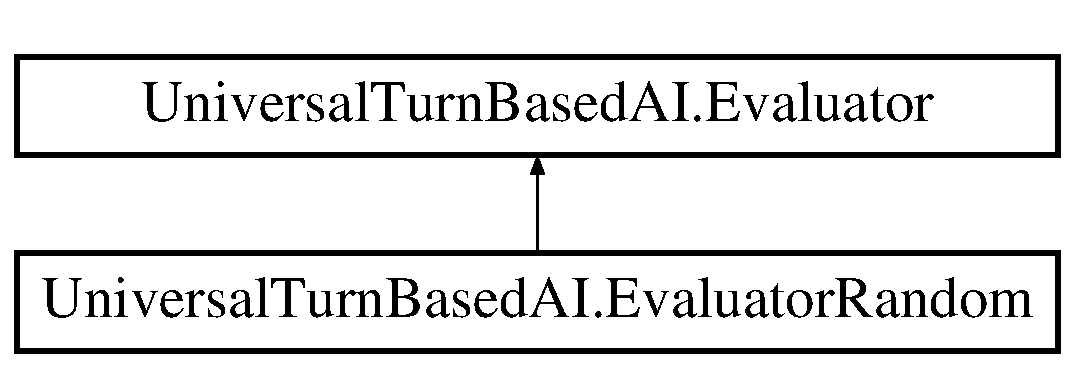
\includegraphics[height=2.000000cm]{class_universal_turn_based_a_i_1_1_evaluator}
\end{center}
\end{figure}
\subsection*{Public Member Functions}
\begin{DoxyCompactItemize}
\item 
abstract float \hyperlink{class_universal_turn_based_a_i_1_1_evaluator_a949d4c3583870a45dc136f1e46114c99}{Evaluate} (\hyperlink{class_universal_turn_based_a_i_1_1_game_state}{Game\+State} state)
\begin{DoxyCompactList}\small\item\em Evaluate the specified \hyperlink{class_universal_turn_based_a_i_1_1_game_state}{Game\+State}. Good evaluation functions should return max\+Value on a winning state and min\+Value on a losing state. This method must also provide value to non-\/terminal states that give the engine some indication of whether the player is closer or further away from winning. \end{DoxyCompactList}\item 
\hypertarget{class_universal_turn_based_a_i_1_1_evaluator_a6cd4b0d6b6e418edd1af8b524cd9b32b}{}abstract \hyperlink{class_universal_turn_based_a_i_1_1_evaluator}{Evaluator} {\bfseries Clone} ()\label{class_universal_turn_based_a_i_1_1_evaluator_a6cd4b0d6b6e418edd1af8b524cd9b32b}

\end{DoxyCompactItemize}
\subsection*{Public Attributes}
\begin{DoxyCompactItemize}
\item 
\hypertarget{class_universal_turn_based_a_i_1_1_evaluator_af1303b4366709d7a5af2fb6e133791fa}{}float {\bfseries min\+Value} = float.\+Min\+Value\label{class_universal_turn_based_a_i_1_1_evaluator_af1303b4366709d7a5af2fb6e133791fa}

\item 
\hypertarget{class_universal_turn_based_a_i_1_1_evaluator_aaa3848cf79994e5674487eb1c6f0f796}{}float {\bfseries max\+Value} = float.\+Max\+Value\label{class_universal_turn_based_a_i_1_1_evaluator_aaa3848cf79994e5674487eb1c6f0f796}

\end{DoxyCompactItemize}


\subsection{Detailed Description}
The super-\/class for all Evaluators. An \hyperlink{class_universal_turn_based_a_i_1_1_evaluator}{Evaluator} defines an evaluation function to determine the value of a \hyperlink{class_universal_turn_based_a_i_1_1_game_state}{Game\+State} from the point of view of a particular player. 

\begin{DoxySeeAlso}{See also}
\hyperlink{class_universal_turn_based_a_i_1_1_turn_engine}{Turn\+Engine}, \hyperlink{class_universal_turn_based_a_i_1_1_game_state}{Game\+State}, \hyperlink{class_universal_turn_based_a_i_1_1_turn}{Turn}


\end{DoxySeeAlso}


\subsection{Member Function Documentation}
\hypertarget{class_universal_turn_based_a_i_1_1_evaluator_a949d4c3583870a45dc136f1e46114c99}{}\index{Universal\+Turn\+Based\+A\+I\+::\+Evaluator@{Universal\+Turn\+Based\+A\+I\+::\+Evaluator}!Evaluate@{Evaluate}}
\index{Evaluate@{Evaluate}!Universal\+Turn\+Based\+A\+I\+::\+Evaluator@{Universal\+Turn\+Based\+A\+I\+::\+Evaluator}}
\subsubsection[{Evaluate}]{\setlength{\rightskip}{0pt plus 5cm}abstract float Universal\+Turn\+Based\+A\+I.\+Evaluator.\+Evaluate (
\begin{DoxyParamCaption}
\item[{{\bf Game\+State}}]{state}
\end{DoxyParamCaption}
)\hspace{0.3cm}{\ttfamily [pure virtual]}}\label{class_universal_turn_based_a_i_1_1_evaluator_a949d4c3583870a45dc136f1e46114c99}


Evaluate the specified \hyperlink{class_universal_turn_based_a_i_1_1_game_state}{Game\+State}. Good evaluation functions should return max\+Value on a winning state and min\+Value on a losing state. This method must also provide value to non-\/terminal states that give the engine some indication of whether the player is closer or further away from winning. 

As this will need to be called on every searched \hyperlink{class_universal_turn_based_a_i_1_1_game_state}{Game\+State} the efficiency of this method is directly related to the performance of a \hyperlink{class_universal_turn_based_a_i_1_1_turn_engine}{Turn\+Engine}. 


\begin{DoxyParams}{Parameters}
{\em state} & The state to evaluate\\
\hline
\end{DoxyParams}


Implemented in \hyperlink{class_universal_turn_based_a_i_1_1_evaluator_random_ac7248adff1c997e43c63e4f34fc3121c}{Universal\+Turn\+Based\+A\+I.\+Evaluator\+Random}.



The documentation for this class was generated from the following file\+:\begin{DoxyCompactItemize}
\item 
Generic\+Turn\+Based\+A\+I/Evaluator.\+cs\end{DoxyCompactItemize}

\hypertarget{class_universal_turn_based_a_i_1_1_evaluator_random}{}\section{Universal\+Turn\+Based\+A\+I.\+Evaluator\+Random Class Reference}
\label{class_universal_turn_based_a_i_1_1_evaluator_random}\index{Universal\+Turn\+Based\+A\+I.\+Evaluator\+Random@{Universal\+Turn\+Based\+A\+I.\+Evaluator\+Random}}


An \hyperlink{class_universal_turn_based_a_i_1_1_evaluator}{Evaluator} that returns random values for every state. Can be useful to test other evaluation functions. Any evaluation function should be at least as good as selecting moves randomly.  


Inheritance diagram for Universal\+Turn\+Based\+A\+I.\+Evaluator\+Random\+:\begin{figure}[H]
\begin{center}
\leavevmode
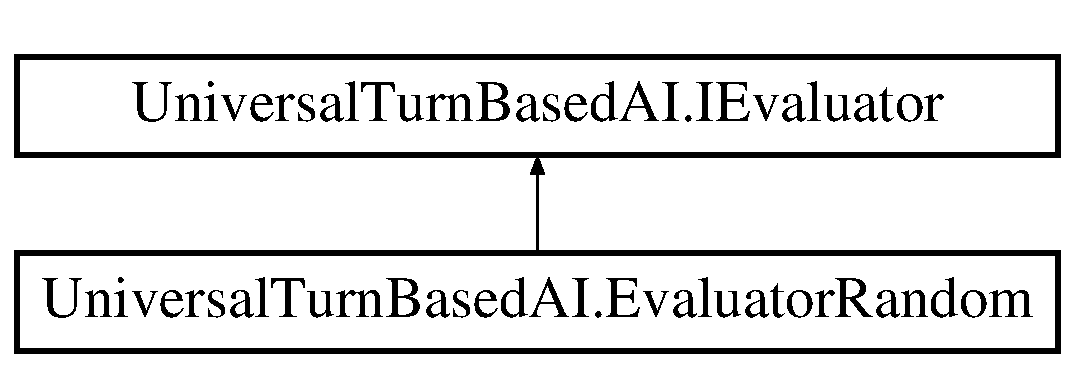
\includegraphics[height=2.000000cm]{class_universal_turn_based_a_i_1_1_evaluator_random}
\end{center}
\end{figure}
\subsection*{Public Member Functions}
\begin{DoxyCompactItemize}
\item 
\hyperlink{class_universal_turn_based_a_i_1_1_evaluator_random_a3914def8b2e2bb2f6a264a6762b84063}{Evaluator\+Random} (float min, float max)
\begin{DoxyCompactList}\small\item\em Initializes a new instance of the \hyperlink{class_universal_turn_based_a_i_1_1_evaluator_random}{Universal\+Turn\+Based\+A\+I.\+Evaluator\+Random} class. \end{DoxyCompactList}\item 
override float \hyperlink{class_universal_turn_based_a_i_1_1_evaluator_random_ac7248adff1c997e43c63e4f34fc3121c}{Evaluate} (\hyperlink{class_universal_turn_based_a_i_1_1_game_state}{Game\+State} state)
\begin{DoxyCompactList}\small\item\em Evaluate the specified \hyperlink{class_universal_turn_based_a_i_1_1_game_state}{Game\+State}. Good evaluation functions should return max\+Value on a winning state and min\+Value on a losing state. This method must also provide value to non-\/terminal states that give the engine some indication of whether the player is closer or further away from winning. \end{DoxyCompactList}\item 
\hypertarget{class_universal_turn_based_a_i_1_1_evaluator_random_a15c6ccc02b7939167f538f82643139bd}{}override \hyperlink{class_universal_turn_based_a_i_1_1_evaluator}{Evaluator} {\bfseries Clone} ()\label{class_universal_turn_based_a_i_1_1_evaluator_random_a15c6ccc02b7939167f538f82643139bd}

\end{DoxyCompactItemize}
\subsection*{Additional Inherited Members}


\subsection{Detailed Description}
An \hyperlink{class_universal_turn_based_a_i_1_1_evaluator}{Evaluator} that returns random values for every state. Can be useful to test other evaluation functions. Any evaluation function should be at least as good as selecting moves randomly. 



\subsection{Constructor \& Destructor Documentation}
\hypertarget{class_universal_turn_based_a_i_1_1_evaluator_random_a3914def8b2e2bb2f6a264a6762b84063}{}\index{Universal\+Turn\+Based\+A\+I\+::\+Evaluator\+Random@{Universal\+Turn\+Based\+A\+I\+::\+Evaluator\+Random}!Evaluator\+Random@{Evaluator\+Random}}
\index{Evaluator\+Random@{Evaluator\+Random}!Universal\+Turn\+Based\+A\+I\+::\+Evaluator\+Random@{Universal\+Turn\+Based\+A\+I\+::\+Evaluator\+Random}}
\subsubsection[{Evaluator\+Random}]{\setlength{\rightskip}{0pt plus 5cm}Universal\+Turn\+Based\+A\+I.\+Evaluator\+Random.\+Evaluator\+Random (
\begin{DoxyParamCaption}
\item[{float}]{min, }
\item[{float}]{max}
\end{DoxyParamCaption}
)\hspace{0.3cm}{\ttfamily [inline]}}\label{class_universal_turn_based_a_i_1_1_evaluator_random_a3914def8b2e2bb2f6a264a6762b84063}


Initializes a new instance of the \hyperlink{class_universal_turn_based_a_i_1_1_evaluator_random}{Universal\+Turn\+Based\+A\+I.\+Evaluator\+Random} class. 


\begin{DoxyParams}{Parameters}
{\em min} & The minimum value to generate\\
\hline
{\em max} & The maximum value to generate\\
\hline
\end{DoxyParams}


\subsection{Member Function Documentation}
\hypertarget{class_universal_turn_based_a_i_1_1_evaluator_random_ac7248adff1c997e43c63e4f34fc3121c}{}\index{Universal\+Turn\+Based\+A\+I\+::\+Evaluator\+Random@{Universal\+Turn\+Based\+A\+I\+::\+Evaluator\+Random}!Evaluate@{Evaluate}}
\index{Evaluate@{Evaluate}!Universal\+Turn\+Based\+A\+I\+::\+Evaluator\+Random@{Universal\+Turn\+Based\+A\+I\+::\+Evaluator\+Random}}
\subsubsection[{Evaluate}]{\setlength{\rightskip}{0pt plus 5cm}override float Universal\+Turn\+Based\+A\+I.\+Evaluator\+Random.\+Evaluate (
\begin{DoxyParamCaption}
\item[{{\bf Game\+State}}]{state}
\end{DoxyParamCaption}
)\hspace{0.3cm}{\ttfamily [inline]}, {\ttfamily [virtual]}}\label{class_universal_turn_based_a_i_1_1_evaluator_random_ac7248adff1c997e43c63e4f34fc3121c}


Evaluate the specified \hyperlink{class_universal_turn_based_a_i_1_1_game_state}{Game\+State}. Good evaluation functions should return max\+Value on a winning state and min\+Value on a losing state. This method must also provide value to non-\/terminal states that give the engine some indication of whether the player is closer or further away from winning. 

As this will need to be called on every searched \hyperlink{class_universal_turn_based_a_i_1_1_game_state}{Game\+State} the efficiency of this method is directly related to the performance of a \hyperlink{class_universal_turn_based_a_i_1_1_turn_engine}{Turn\+Engine}. 


\begin{DoxyParams}{Parameters}
{\em state} & The state to evaluate\\
\hline
\end{DoxyParams}


Implements \hyperlink{class_universal_turn_based_a_i_1_1_evaluator_a949d4c3583870a45dc136f1e46114c99}{Universal\+Turn\+Based\+A\+I.\+Evaluator}.



The documentation for this class was generated from the following file\+:\begin{DoxyCompactItemize}
\item 
Generic\+Turn\+Based\+A\+I/Evaluator\+Random.\+cs\end{DoxyCompactItemize}

\hypertarget{class_universal_turn_based_a_i_1_1_game_state}{}\section{Universal\+Turn\+Based\+A\+I.\+Game\+State Class Reference}
\label{class_universal_turn_based_a_i_1_1_game_state}\index{Universal\+Turn\+Based\+A\+I.\+Game\+State@{Universal\+Turn\+Based\+A\+I.\+Game\+State}}


The super-\/class for Game\+States. Represents the current state of some game. Implement this class to provide a \hyperlink{class_universal_turn_based_a_i_1_1_turn_engine}{Turn\+Engine} with domain specific knowledge. The effiency of \hyperlink{class_universal_turn_based_a_i_1_1_game_state_a2d877d322bd57b7c6962d09b20baeebb}{Is\+Terminal}, \hyperlink{class_universal_turn_based_a_i_1_1_game_state_a252554bfd9fd58bdc06bd6f49b716240}{Generate\+Possible\+Turns} and \hyperlink{class_universal_turn_based_a_i_1_1_game_state_a7e9d117069df3da5b42eeadecf33a326}{Clone} will all effect the performance of the \hyperlink{class_universal_turn_based_a_i_1_1_turn_engine}{Turn\+Engine}.  


\subsection*{Public Member Functions}
\begin{DoxyCompactItemize}
\item 
abstract bool \hyperlink{class_universal_turn_based_a_i_1_1_game_state_a2d877d322bd57b7c6962d09b20baeebb}{Is\+Terminal} ()
\begin{DoxyCompactList}\small\item\em Determines whether this \hyperlink{class_universal_turn_based_a_i_1_1_game_state}{Game\+State} is terminal. \end{DoxyCompactList}\item 
abstract I\+Enumerable$<$ \hyperlink{class_universal_turn_based_a_i_1_1_turn}{Turn} $>$ \hyperlink{class_universal_turn_based_a_i_1_1_game_state_a252554bfd9fd58bdc06bd6f49b716240}{Generate\+Possible\+Turns} ()
\begin{DoxyCompactList}\small\item\em A coroutine for generating every possible \hyperlink{class_universal_turn_based_a_i_1_1_turn}{Turn}. Generating turns this way allows turns to be generated and search lazily. The efficiency of generating each turn effects the performance of the \hyperlink{class_universal_turn_based_a_i_1_1_turn_engine}{Turn\+Engine}. You will only get the benefits of lazy evaluation if you yield each turn after generating them. Generating all turns and then iterating through them will negatively effect the performance of the \hyperlink{class_universal_turn_based_a_i_1_1_turn_engine}{Turn\+Engine}. \end{DoxyCompactList}\item 
abstract \hyperlink{class_universal_turn_based_a_i_1_1_game_state}{Game\+State} \hyperlink{class_universal_turn_based_a_i_1_1_game_state_a7e9d117069df3da5b42eeadecf33a326}{Clone} ()
\begin{DoxyCompactList}\small\item\em Returns an exact copy of the current \hyperlink{class_universal_turn_based_a_i_1_1_game_state}{Game\+State} with new references. Any \hyperlink{class_universal_turn_based_a_i_1_1_game_state}{Game\+State} information that is altered by a \hyperlink{class_universal_turn_based_a_i_1_1_turn}{Turn} should be deep copied to prevent Turns writing over shared information. \end{DoxyCompactList}\end{DoxyCompactItemize}


\subsection{Detailed Description}
The super-\/class for Game\+States. Represents the current state of some game. Implement this class to provide a \hyperlink{class_universal_turn_based_a_i_1_1_turn_engine}{Turn\+Engine} with domain specific knowledge. The effiency of \hyperlink{class_universal_turn_based_a_i_1_1_game_state_a2d877d322bd57b7c6962d09b20baeebb}{Is\+Terminal}, \hyperlink{class_universal_turn_based_a_i_1_1_game_state_a252554bfd9fd58bdc06bd6f49b716240}{Generate\+Possible\+Turns} and \hyperlink{class_universal_turn_based_a_i_1_1_game_state_a7e9d117069df3da5b42eeadecf33a326}{Clone} will all effect the performance of the \hyperlink{class_universal_turn_based_a_i_1_1_turn_engine}{Turn\+Engine}. 

Some information that is typically useful is\+: whose turn it is and some representation of the state of each component of the game. It can also be useful to track some meta-\/information about the state that can be used by an evaluation function rather than having the evaluation function compute the information every time. For example, counts of things within the \hyperlink{class_universal_turn_based_a_i_1_1_game_state}{Game\+State}. \begin{DoxySeeAlso}{See also}
\hyperlink{class_universal_turn_based_a_i_1_1_turn_engine}{Turn\+Engine}, \hyperlink{class_universal_turn_based_a_i_1_1_turn}{Turn}, \hyperlink{class_universal_turn_based_a_i_1_1_evaluator}{Evaluator}


\end{DoxySeeAlso}


\subsection{Member Function Documentation}
\hypertarget{class_universal_turn_based_a_i_1_1_game_state_a7e9d117069df3da5b42eeadecf33a326}{}\index{Universal\+Turn\+Based\+A\+I\+::\+Game\+State@{Universal\+Turn\+Based\+A\+I\+::\+Game\+State}!Clone@{Clone}}
\index{Clone@{Clone}!Universal\+Turn\+Based\+A\+I\+::\+Game\+State@{Universal\+Turn\+Based\+A\+I\+::\+Game\+State}}
\subsubsection[{Clone}]{\setlength{\rightskip}{0pt plus 5cm}abstract {\bf Game\+State} Universal\+Turn\+Based\+A\+I.\+Game\+State.\+Clone (
\begin{DoxyParamCaption}
{}
\end{DoxyParamCaption}
)\hspace{0.3cm}{\ttfamily [pure virtual]}}\label{class_universal_turn_based_a_i_1_1_game_state_a7e9d117069df3da5b42eeadecf33a326}


Returns an exact copy of the current \hyperlink{class_universal_turn_based_a_i_1_1_game_state}{Game\+State} with new references. Any \hyperlink{class_universal_turn_based_a_i_1_1_game_state}{Game\+State} information that is altered by a \hyperlink{class_universal_turn_based_a_i_1_1_turn}{Turn} should be deep copied to prevent Turns writing over shared information. 

The efficiency of this method effects the performance of the \hyperlink{class_universal_turn_based_a_i_1_1_turn_engine}{Turn\+Engine}, try to copy as little information as possible but remember that you will probably need new instances of any reference types that can be altered by a \hyperlink{class_universal_turn_based_a_i_1_1_turn}{Turn}. \hypertarget{class_universal_turn_based_a_i_1_1_game_state_a252554bfd9fd58bdc06bd6f49b716240}{}\index{Universal\+Turn\+Based\+A\+I\+::\+Game\+State@{Universal\+Turn\+Based\+A\+I\+::\+Game\+State}!Generate\+Possible\+Turns@{Generate\+Possible\+Turns}}
\index{Generate\+Possible\+Turns@{Generate\+Possible\+Turns}!Universal\+Turn\+Based\+A\+I\+::\+Game\+State@{Universal\+Turn\+Based\+A\+I\+::\+Game\+State}}
\subsubsection[{Generate\+Possible\+Turns}]{\setlength{\rightskip}{0pt plus 5cm}abstract I\+Enumerable$<${\bf Turn}$>$ Universal\+Turn\+Based\+A\+I.\+Game\+State.\+Generate\+Possible\+Turns (
\begin{DoxyParamCaption}
{}
\end{DoxyParamCaption}
)\hspace{0.3cm}{\ttfamily [pure virtual]}}\label{class_universal_turn_based_a_i_1_1_game_state_a252554bfd9fd58bdc06bd6f49b716240}


A coroutine for generating every possible \hyperlink{class_universal_turn_based_a_i_1_1_turn}{Turn}. Generating turns this way allows turns to be generated and search lazily. The efficiency of generating each turn effects the performance of the \hyperlink{class_universal_turn_based_a_i_1_1_turn_engine}{Turn\+Engine}. You will only get the benefits of lazy evaluation if you yield each turn after generating them. Generating all turns and then iterating through them will negatively effect the performance of the \hyperlink{class_universal_turn_based_a_i_1_1_turn_engine}{Turn\+Engine}. 

This method should only produce turns that are valid for this particular \hyperlink{class_universal_turn_based_a_i_1_1_game_state}{Game\+State} 

\begin{DoxyReturn}{Returns}
The possible turns.
\end{DoxyReturn}
\hypertarget{class_universal_turn_based_a_i_1_1_game_state_a2d877d322bd57b7c6962d09b20baeebb}{}\index{Universal\+Turn\+Based\+A\+I\+::\+Game\+State@{Universal\+Turn\+Based\+A\+I\+::\+Game\+State}!Is\+Terminal@{Is\+Terminal}}
\index{Is\+Terminal@{Is\+Terminal}!Universal\+Turn\+Based\+A\+I\+::\+Game\+State@{Universal\+Turn\+Based\+A\+I\+::\+Game\+State}}
\subsubsection[{Is\+Terminal}]{\setlength{\rightskip}{0pt plus 5cm}abstract bool Universal\+Turn\+Based\+A\+I.\+Game\+State.\+Is\+Terminal (
\begin{DoxyParamCaption}
{}
\end{DoxyParamCaption}
)\hspace{0.3cm}{\ttfamily [pure virtual]}}\label{class_universal_turn_based_a_i_1_1_game_state_a2d877d322bd57b7c6962d09b20baeebb}


Determines whether this \hyperlink{class_universal_turn_based_a_i_1_1_game_state}{Game\+State} is terminal. 

\begin{DoxyReturn}{Returns}
{\ttfamily true} If this \hyperlink{class_universal_turn_based_a_i_1_1_game_state}{Game\+State} is terminal; otherwise, {\ttfamily false}.
\end{DoxyReturn}


The documentation for this class was generated from the following file\+:\begin{DoxyCompactItemize}
\item 
Generic\+Turn\+Based\+A\+I/Game\+State.\+cs\end{DoxyCompactItemize}

\hypertarget{class_universal_turn_based_a_i_1_1_minimax_worker}{}\section{Universal\+Turn\+Based\+A\+I.\+Minimax\+Worker Class Reference}
\label{class_universal_turn_based_a_i_1_1_minimax_worker}\index{Universal\+Turn\+Based\+A\+I.\+Minimax\+Worker@{Universal\+Turn\+Based\+A\+I.\+Minimax\+Worker}}


Holds all of the initialising information required for a Minimax search so it can more easily be passed to a Thread\+Pool  


\subsection*{Public Member Functions}
\begin{DoxyCompactItemize}
\item 
\hyperlink{class_universal_turn_based_a_i_1_1_minimax_worker_aefc299364d8cbc30ebb6caba179703d7}{Minimax\+Worker} (\hyperlink{interface_universal_turn_based_a_i_1_1_i_game_state}{I\+Game\+State} root\+State, \hyperlink{interface_universal_turn_based_a_i_1_1_i_turn}{I\+Turn} \hyperlink{class_universal_turn_based_a_i_1_1_minimax_worker_a7b1186503a4def5fa695b58502d05c9b}{first\+Turn}, \hyperlink{interface_universal_turn_based_a_i_1_1_i_evaluator}{I\+Evaluator} eval, int max\+Depth, bool our\+Turn, Event\+Wait\+Handle wait\+Handle)
\begin{DoxyCompactList}\small\item\em Initializes a new instance of the \hyperlink{class_universal_turn_based_a_i_1_1_minimax_worker}{Universal\+Turn\+Based\+A\+I.\+Minimax\+Worker} class. \end{DoxyCompactList}\item 
\hypertarget{class_universal_turn_based_a_i_1_1_minimax_worker_a3003a7a26d65f3e6ef877f21c7c7d307}{}void {\bfseries Evaluate\+State} (object thread\+State)\label{class_universal_turn_based_a_i_1_1_minimax_worker_a3003a7a26d65f3e6ef877f21c7c7d307}

\item 
\hypertarget{class_universal_turn_based_a_i_1_1_minimax_worker_ad9b6596f36acc2970d865c8b4a29d882}{}float {\bfseries Alpha\+Beta} (\hyperlink{interface_universal_turn_based_a_i_1_1_i_game_state}{I\+Game\+State} state, \hyperlink{interface_universal_turn_based_a_i_1_1_i_evaluator}{I\+Evaluator} eval, int depth, float alpha, float beta, bool our\+Turn)\label{class_universal_turn_based_a_i_1_1_minimax_worker_ad9b6596f36acc2970d865c8b4a29d882}

\item 
\hypertarget{class_universal_turn_based_a_i_1_1_minimax_worker_aaf19d669a25879a067716e12af1326be}{}void {\bfseries Stop} ()\label{class_universal_turn_based_a_i_1_1_minimax_worker_aaf19d669a25879a067716e12af1326be}

\end{DoxyCompactItemize}
\subsection*{Public Attributes}
\begin{DoxyCompactItemize}
\item 
\hyperlink{interface_universal_turn_based_a_i_1_1_i_turn}{I\+Turn} \hyperlink{class_universal_turn_based_a_i_1_1_minimax_worker_a7b1186503a4def5fa695b58502d05c9b}{first\+Turn}
\begin{DoxyCompactList}\small\item\em The first turn to use in the search this is the turn retrieved for returning \end{DoxyCompactList}\end{DoxyCompactItemize}
\subsection*{Properties}
\begin{DoxyCompactItemize}
\item 
float \hyperlink{class_universal_turn_based_a_i_1_1_minimax_worker_aba59322c19f8226090dfaf8d7b5d8737}{Value}\hspace{0.3cm}{\ttfamily  \mbox{[}get\mbox{]}}
\begin{DoxyCompactList}\small\item\em The value of {\itshape first\+Turn}  \end{DoxyCompactList}\end{DoxyCompactItemize}


\subsection{Detailed Description}
Holds all of the initialising information required for a Minimax search so it can more easily be passed to a Thread\+Pool 



\subsection{Constructor \& Destructor Documentation}
\hypertarget{class_universal_turn_based_a_i_1_1_minimax_worker_aefc299364d8cbc30ebb6caba179703d7}{}\index{Universal\+Turn\+Based\+A\+I\+::\+Minimax\+Worker@{Universal\+Turn\+Based\+A\+I\+::\+Minimax\+Worker}!Minimax\+Worker@{Minimax\+Worker}}
\index{Minimax\+Worker@{Minimax\+Worker}!Universal\+Turn\+Based\+A\+I\+::\+Minimax\+Worker@{Universal\+Turn\+Based\+A\+I\+::\+Minimax\+Worker}}
\subsubsection[{Minimax\+Worker}]{\setlength{\rightskip}{0pt plus 5cm}Universal\+Turn\+Based\+A\+I.\+Minimax\+Worker.\+Minimax\+Worker (
\begin{DoxyParamCaption}
\item[{{\bf I\+Game\+State}}]{root\+State, }
\item[{{\bf I\+Turn}}]{first\+Turn, }
\item[{{\bf I\+Evaluator}}]{eval, }
\item[{int}]{max\+Depth, }
\item[{bool}]{our\+Turn, }
\item[{Event\+Wait\+Handle}]{wait\+Handle}
\end{DoxyParamCaption}
)\hspace{0.3cm}{\ttfamily [inline]}}\label{class_universal_turn_based_a_i_1_1_minimax_worker_aefc299364d8cbc30ebb6caba179703d7}


Initializes a new instance of the \hyperlink{class_universal_turn_based_a_i_1_1_minimax_worker}{Universal\+Turn\+Based\+A\+I.\+Minimax\+Worker} class. 


\begin{DoxyParams}{Parameters}
{\em root\+State} & The starting state\\
\hline
{\em first\+Turn} & The turn to apply to the starting state to generate this worker\textquotesingle{}s branch\\
\hline
{\em eval} & The Evaluator\\
\hline
{\em max\+Depth} & Max depth.\\
\hline
{\em our\+Turn} & Whether or not it is the searching player\textquotesingle{}s turn\\
\hline
{\em wait\+Handle} & Signals the Thread\+Pool that the search is complete\\
\hline
\end{DoxyParams}


\subsection{Member Data Documentation}
\hypertarget{class_universal_turn_based_a_i_1_1_minimax_worker_a7b1186503a4def5fa695b58502d05c9b}{}\index{Universal\+Turn\+Based\+A\+I\+::\+Minimax\+Worker@{Universal\+Turn\+Based\+A\+I\+::\+Minimax\+Worker}!first\+Turn@{first\+Turn}}
\index{first\+Turn@{first\+Turn}!Universal\+Turn\+Based\+A\+I\+::\+Minimax\+Worker@{Universal\+Turn\+Based\+A\+I\+::\+Minimax\+Worker}}
\subsubsection[{first\+Turn}]{\setlength{\rightskip}{0pt plus 5cm}{\bf I\+Turn} Universal\+Turn\+Based\+A\+I.\+Minimax\+Worker.\+first\+Turn}\label{class_universal_turn_based_a_i_1_1_minimax_worker_a7b1186503a4def5fa695b58502d05c9b}


The first turn to use in the search this is the turn retrieved for returning 



\subsection{Property Documentation}
\hypertarget{class_universal_turn_based_a_i_1_1_minimax_worker_aba59322c19f8226090dfaf8d7b5d8737}{}\index{Universal\+Turn\+Based\+A\+I\+::\+Minimax\+Worker@{Universal\+Turn\+Based\+A\+I\+::\+Minimax\+Worker}!Value@{Value}}
\index{Value@{Value}!Universal\+Turn\+Based\+A\+I\+::\+Minimax\+Worker@{Universal\+Turn\+Based\+A\+I\+::\+Minimax\+Worker}}
\subsubsection[{Value}]{\setlength{\rightskip}{0pt plus 5cm}float Universal\+Turn\+Based\+A\+I.\+Minimax\+Worker.\+Value\hspace{0.3cm}{\ttfamily [get]}}\label{class_universal_turn_based_a_i_1_1_minimax_worker_aba59322c19f8226090dfaf8d7b5d8737}


The value of {\itshape first\+Turn}  

The value.

The documentation for this class was generated from the following file\+:\begin{DoxyCompactItemize}
\item 
Generic\+Turn\+Based\+A\+I/Minimax\+Worker.\+cs\end{DoxyCompactItemize}

\hypertarget{class_universal_turn_based_a_i_1_1_turn}{}\section{Universal\+Turn\+Based\+A\+I.\+Turn Class Reference}
\label{class_universal_turn_based_a_i_1_1_turn}\index{Universal\+Turn\+Based\+A\+I.\+Turn@{Universal\+Turn\+Based\+A\+I.\+Turn}}


A super-\/class for Turns. Represents the sum of actions that a player can take on their turn in the game.  


\subsection*{Public Member Functions}
\begin{DoxyCompactItemize}
\item 
abstract \hyperlink{class_universal_turn_based_a_i_1_1_game_state}{Game\+State} \hyperlink{class_universal_turn_based_a_i_1_1_turn_aa28ba0a68683fda933158b242c683b22}{Apply\+Turn} (\hyperlink{class_universal_turn_based_a_i_1_1_game_state}{Game\+State} state)
\begin{DoxyCompactList}\small\item\em Applies this \hyperlink{class_universal_turn_based_a_i_1_1_turn}{Turn} to {\itshape state}  giving the resulting \hyperlink{class_universal_turn_based_a_i_1_1_game_state}{Game\+State}. The \hyperlink{class_universal_turn_based_a_i_1_1_turn_engine}{Turn\+Engine} clones {\itshape state}  before passing it to this function when called internally to prevent the original \hyperlink{class_universal_turn_based_a_i_1_1_game_state}{Game\+State} from being overridden \begin{DoxySeeAlso}{See also}
\hyperlink{class_universal_turn_based_a_i_1_1_game_state}{Game\+State}, \hyperlink{class_universal_turn_based_a_i_1_1_turn_engine}{Turn\+Engine}


\end{DoxySeeAlso}
\end{DoxyCompactList}\end{DoxyCompactItemize}


\subsection{Detailed Description}
A super-\/class for Turns. Represents the sum of actions that a player can take on their turn in the game. 

\begin{DoxySeeAlso}{See also}
\hyperlink{class_universal_turn_based_a_i_1_1_game_state}{Game\+State}, \hyperlink{class_universal_turn_based_a_i_1_1_turn_engine}{Turn\+Engine}


\end{DoxySeeAlso}


\subsection{Member Function Documentation}
\hypertarget{class_universal_turn_based_a_i_1_1_turn_aa28ba0a68683fda933158b242c683b22}{}\index{Universal\+Turn\+Based\+A\+I\+::\+Turn@{Universal\+Turn\+Based\+A\+I\+::\+Turn}!Apply\+Turn@{Apply\+Turn}}
\index{Apply\+Turn@{Apply\+Turn}!Universal\+Turn\+Based\+A\+I\+::\+Turn@{Universal\+Turn\+Based\+A\+I\+::\+Turn}}
\subsubsection[{Apply\+Turn}]{\setlength{\rightskip}{0pt plus 5cm}abstract {\bf Game\+State} Universal\+Turn\+Based\+A\+I.\+Turn.\+Apply\+Turn (
\begin{DoxyParamCaption}
\item[{{\bf Game\+State}}]{state}
\end{DoxyParamCaption}
)\hspace{0.3cm}{\ttfamily [pure virtual]}}\label{class_universal_turn_based_a_i_1_1_turn_aa28ba0a68683fda933158b242c683b22}


Applies this \hyperlink{class_universal_turn_based_a_i_1_1_turn}{Turn} to {\itshape state}  giving the resulting \hyperlink{class_universal_turn_based_a_i_1_1_game_state}{Game\+State}. The \hyperlink{class_universal_turn_based_a_i_1_1_turn_engine}{Turn\+Engine} clones {\itshape state}  before passing it to this function when called internally to prevent the original \hyperlink{class_universal_turn_based_a_i_1_1_game_state}{Game\+State} from being overridden \begin{DoxySeeAlso}{See also}
\hyperlink{class_universal_turn_based_a_i_1_1_game_state}{Game\+State}, \hyperlink{class_universal_turn_based_a_i_1_1_turn_engine}{Turn\+Engine}


\end{DoxySeeAlso}


\begin{DoxyReturn}{Returns}
The \hyperlink{class_universal_turn_based_a_i_1_1_game_state}{Game\+State} that is a result of applying this turn to {\itshape state} .
\end{DoxyReturn}

\begin{DoxyParams}{Parameters}
{\em state} & The state to apply the turn to.\\
\hline
\end{DoxyParams}


The documentation for this class was generated from the following file\+:\begin{DoxyCompactItemize}
\item 
Generic\+Turn\+Based\+A\+I/Turn.\+cs\end{DoxyCompactItemize}

\hypertarget{class_universal_turn_based_a_i_1_1_turn_engine}{}\section{Universal\+Turn\+Based\+A\+I.\+Turn\+Engine Class Reference}
\label{class_universal_turn_based_a_i_1_1_turn_engine}\index{Universal\+Turn\+Based\+A\+I.\+Turn\+Engine@{Universal\+Turn\+Based\+A\+I.\+Turn\+Engine}}


The super-\/class for all Turn Engines. Implementations of this class control the search for the best \hyperlink{interface_universal_turn_based_a_i_1_1_i_turn}{I\+Turn}. Provides an entry point for Unity with \hyperlink{class_universal_turn_based_a_i_1_1_turn_engine_ad1a07e70064e2f188b65a783aa49cd8a}{Get\+Next\+Turn} which can be used in a familiar coroutine pattern. Defines attributes common to all Turn Engines such as depth and time limits. Also provides the \hyperlink{class_universal_turn_based_a_i_1_1_turn_engine_af10115494121382d2966a8fc9fe4c9a0}{Turn\+Ready\+Event} which is triggered after a turn search has been completed and returns the best turn found.  


Inheritance diagram for Universal\+Turn\+Based\+A\+I.\+Turn\+Engine\+:\begin{figure}[H]
\begin{center}
\leavevmode
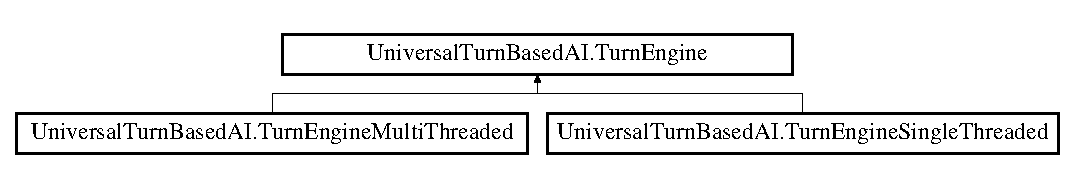
\includegraphics[height=1.842105cm]{class_universal_turn_based_a_i_1_1_turn_engine}
\end{center}
\end{figure}
\subsection*{Public Member Functions}
\begin{DoxyCompactItemize}
\item 
\hypertarget{class_universal_turn_based_a_i_1_1_turn_engine_a8e529eaca1c650dc031b151b381242b5}{}delegate void {\bfseries Turn\+Ready} (\hyperlink{interface_universal_turn_based_a_i_1_1_i_turn}{I\+Turn} best\+Turn)\label{class_universal_turn_based_a_i_1_1_turn_engine_a8e529eaca1c650dc031b151b381242b5}

\item 
System.\+Collections.\+I\+Enumerator \hyperlink{class_universal_turn_based_a_i_1_1_turn_engine_ad1a07e70064e2f188b65a783aa49cd8a}{Get\+Next\+Turn} (\hyperlink{interface_universal_turn_based_a_i_1_1_i_game_state}{I\+Game\+State} state)
\begin{DoxyCompactList}\small\item\em The entry point to the engine. Starts a new thread to run the search in and waits on it. Once the search is completed or timed out, calls the \hyperlink{class_universal_turn_based_a_i_1_1_turn_engine_af10115494121382d2966a8fc9fe4c9a0}{Turn\+Ready\+Event} to return the best turn found. \end{DoxyCompactList}\item 
\hypertarget{class_universal_turn_based_a_i_1_1_turn_engine_a210fed5125af320ef0a9634305bca467}{}\hyperlink{class_universal_turn_based_a_i_1_1_engine_stats}{Engine\+Stats} {\bfseries Reset\+Statistics\+Log} ()\label{class_universal_turn_based_a_i_1_1_turn_engine_a210fed5125af320ef0a9634305bca467}

\item 
\hypertarget{class_universal_turn_based_a_i_1_1_turn_engine_a2a1210eb5816e1335f80d7a05efdafbf}{}virtual void {\bfseries Stop} ()\label{class_universal_turn_based_a_i_1_1_turn_engine_a2a1210eb5816e1335f80d7a05efdafbf}

\end{DoxyCompactItemize}
\subsection*{Protected Member Functions}
\begin{DoxyCompactItemize}
\item 
void \hyperlink{class_universal_turn_based_a_i_1_1_turn_engine_aeb42263a4aff0a25e124654af9a9286b}{Init\+Engine} (\hyperlink{interface_universal_turn_based_a_i_1_1_i_evaluator}{I\+Evaluator} eval, float time\+Limit, int depth\+Limit, bool time\+Limited, bool collect\+Stats)
\begin{DoxyCompactList}\small\item\em Initialises the common engine elements. \end{DoxyCompactList}\item 
void \hyperlink{class_universal_turn_based_a_i_1_1_turn_engine_a7b14c450da986c60ebab0d992081371c}{Execute\+And\+Catch} (Action$<$ object $>$ action, object arg, Action$<$ Exception $>$ exception\+Handler)
\begin{DoxyCompactList}\small\item\em Wrapper for catching exceptions from another thread \end{DoxyCompactList}\item 
void \hyperlink{class_universal_turn_based_a_i_1_1_turn_engine_a1d1d7061052986196974028919d5c45f}{Exception\+Handler} (Exception ex)
\begin{DoxyCompactList}\small\item\em Writes .N\+E\+T exceptions to the Unity Debug Log \end{DoxyCompactList}\item 
\hypertarget{class_universal_turn_based_a_i_1_1_turn_engine_af34e85df941ad5c3cb3b1af7260752fe}{}abstract void {\bfseries Turn\+Search\+Delegate} (object state)\label{class_universal_turn_based_a_i_1_1_turn_engine_af34e85df941ad5c3cb3b1af7260752fe}

\end{DoxyCompactItemize}
\subsection*{Static Protected Member Functions}
\begin{DoxyCompactItemize}
\item 
\hypertarget{class_universal_turn_based_a_i_1_1_turn_engine_a2f0108600a38970fa4f8d46ac5919e3d}{}static T {\bfseries Get\+Random\+Element$<$ T $>$} (I\+List$<$ T $>$ list)\label{class_universal_turn_based_a_i_1_1_turn_engine_a2f0108600a38970fa4f8d46ac5919e3d}

\end{DoxyCompactItemize}
\subsection*{Protected Attributes}
\begin{DoxyCompactItemize}
\item 
\hypertarget{class_universal_turn_based_a_i_1_1_turn_engine_a7347274a628ec2ddb7fa6a8406afe881}{}int {\bfseries max\+Depth}\label{class_universal_turn_based_a_i_1_1_turn_engine_a7347274a628ec2ddb7fa6a8406afe881}

\item 
\hypertarget{class_universal_turn_based_a_i_1_1_turn_engine_a40e0506e4c084dd213a01759d1a13802}{}float {\bfseries max\+Time}\label{class_universal_turn_based_a_i_1_1_turn_engine_a40e0506e4c084dd213a01759d1a13802}

\item 
\hypertarget{class_universal_turn_based_a_i_1_1_turn_engine_aa209ad1026c8f043bf2ad358951e795b}{}bool {\bfseries time\+Limited} = false\label{class_universal_turn_based_a_i_1_1_turn_engine_aa209ad1026c8f043bf2ad358951e795b}

\item 
\hypertarget{class_universal_turn_based_a_i_1_1_turn_engine_a7dc55f0df4f72a99a137744fb2865a03}{}\hyperlink{interface_universal_turn_based_a_i_1_1_i_evaluator}{I\+Evaluator} {\bfseries eval}\label{class_universal_turn_based_a_i_1_1_turn_engine_a7dc55f0df4f72a99a137744fb2865a03}

\item 
\hypertarget{class_universal_turn_based_a_i_1_1_turn_engine_ab4a539edefe5953b9954a850a1562a9c}{}System.\+Random {\bfseries rando}\label{class_universal_turn_based_a_i_1_1_turn_engine_ab4a539edefe5953b9954a850a1562a9c}

\item 
\hypertarget{class_universal_turn_based_a_i_1_1_turn_engine_a31430188d6c5d23190c21066a258c7d4}{}Date\+Time {\bfseries start\+Time}\label{class_universal_turn_based_a_i_1_1_turn_engine_a31430188d6c5d23190c21066a258c7d4}

\item 
\hypertarget{class_universal_turn_based_a_i_1_1_turn_engine_a04cfc341ef23a654a3a0028b2db143bb}{}bool {\bfseries collect\+Stats} = false\label{class_universal_turn_based_a_i_1_1_turn_engine_a04cfc341ef23a654a3a0028b2db143bb}

\item 
\hypertarget{class_universal_turn_based_a_i_1_1_turn_engine_a4932da2d4516a3be9af2c240968d3324}{}bool {\bfseries stopped} = true\label{class_universal_turn_based_a_i_1_1_turn_engine_a4932da2d4516a3be9af2c240968d3324}

\item 
\hypertarget{class_universal_turn_based_a_i_1_1_turn_engine_a0d76791b9a154a704d2a5acb9bca529a}{}\hyperlink{interface_universal_turn_based_a_i_1_1_i_turn}{I\+Turn} {\bfseries best\+Turn}\label{class_universal_turn_based_a_i_1_1_turn_engine_a0d76791b9a154a704d2a5acb9bca529a}

\end{DoxyCompactItemize}
\subsection*{Properties}
\begin{DoxyCompactItemize}
\item 
\hyperlink{class_universal_turn_based_a_i_1_1_engine_stats}{Engine\+Stats} \hyperlink{class_universal_turn_based_a_i_1_1_turn_engine_a2588f0e4a11f2c96613e72c890e39138}{Stats}\hspace{0.3cm}{\ttfamily  \mbox{[}get\mbox{]}}
\begin{DoxyCompactList}\small\item\em Property for accessing stats if there were collect. \end{DoxyCompactList}\item 
\hypertarget{class_universal_turn_based_a_i_1_1_turn_engine_aa96090059f46e1c54a9e7edde40c9f2d}{}bool {\bfseries Exit}\hspace{0.3cm}{\ttfamily  \mbox{[}get\mbox{]}}\label{class_universal_turn_based_a_i_1_1_turn_engine_aa96090059f46e1c54a9e7edde40c9f2d}

\end{DoxyCompactItemize}
\subsection*{Events}
\begin{DoxyCompactItemize}
\item 
Turn\+Ready \hyperlink{class_universal_turn_based_a_i_1_1_turn_engine_af10115494121382d2966a8fc9fe4c9a0}{Turn\+Ready\+Event}
\begin{DoxyCompactList}\small\item\em Triggered after \hyperlink{class_universal_turn_based_a_i_1_1_turn_engine_ad1a07e70064e2f188b65a783aa49cd8a}{Get\+Next\+Turn} has been called and the found turn is ready to be returned. best\+Turn will be the best turn discovered by the engine \end{DoxyCompactList}\end{DoxyCompactItemize}


\subsection{Detailed Description}
The super-\/class for all Turn Engines. Implementations of this class control the search for the best \hyperlink{interface_universal_turn_based_a_i_1_1_i_turn}{I\+Turn}. Provides an entry point for Unity with \hyperlink{class_universal_turn_based_a_i_1_1_turn_engine_ad1a07e70064e2f188b65a783aa49cd8a}{Get\+Next\+Turn} which can be used in a familiar coroutine pattern. Defines attributes common to all Turn Engines such as depth and time limits. Also provides the \hyperlink{class_universal_turn_based_a_i_1_1_turn_engine_af10115494121382d2966a8fc9fe4c9a0}{Turn\+Ready\+Event} which is triggered after a turn search has been completed and returns the best turn found. 

\begin{DoxySeeAlso}{See also}
\hyperlink{interface_universal_turn_based_a_i_1_1_i_game_state}{I\+Game\+State}, \hyperlink{interface_universal_turn_based_a_i_1_1_i_turn}{I\+Turn}, \hyperlink{interface_universal_turn_based_a_i_1_1_i_evaluator}{I\+Evaluator}


\end{DoxySeeAlso}


\subsection{Member Function Documentation}
\hypertarget{class_universal_turn_based_a_i_1_1_turn_engine_a1d1d7061052986196974028919d5c45f}{}\index{Universal\+Turn\+Based\+A\+I\+::\+Turn\+Engine@{Universal\+Turn\+Based\+A\+I\+::\+Turn\+Engine}!Exception\+Handler@{Exception\+Handler}}
\index{Exception\+Handler@{Exception\+Handler}!Universal\+Turn\+Based\+A\+I\+::\+Turn\+Engine@{Universal\+Turn\+Based\+A\+I\+::\+Turn\+Engine}}
\subsubsection[{Exception\+Handler}]{\setlength{\rightskip}{0pt plus 5cm}void Universal\+Turn\+Based\+A\+I.\+Turn\+Engine.\+Exception\+Handler (
\begin{DoxyParamCaption}
\item[{Exception}]{ex}
\end{DoxyParamCaption}
)\hspace{0.3cm}{\ttfamily [inline]}, {\ttfamily [protected]}}\label{class_universal_turn_based_a_i_1_1_turn_engine_a1d1d7061052986196974028919d5c45f}


Writes .N\+E\+T exceptions to the Unity Debug Log 


\begin{DoxyParams}{Parameters}
{\em ex} & The exception\\
\hline
\end{DoxyParams}
\hypertarget{class_universal_turn_based_a_i_1_1_turn_engine_a7b14c450da986c60ebab0d992081371c}{}\index{Universal\+Turn\+Based\+A\+I\+::\+Turn\+Engine@{Universal\+Turn\+Based\+A\+I\+::\+Turn\+Engine}!Execute\+And\+Catch@{Execute\+And\+Catch}}
\index{Execute\+And\+Catch@{Execute\+And\+Catch}!Universal\+Turn\+Based\+A\+I\+::\+Turn\+Engine@{Universal\+Turn\+Based\+A\+I\+::\+Turn\+Engine}}
\subsubsection[{Execute\+And\+Catch}]{\setlength{\rightskip}{0pt plus 5cm}void Universal\+Turn\+Based\+A\+I.\+Turn\+Engine.\+Execute\+And\+Catch (
\begin{DoxyParamCaption}
\item[{Action$<$ object $>$}]{action, }
\item[{object}]{arg, }
\item[{Action$<$ Exception $>$}]{exception\+Handler}
\end{DoxyParamCaption}
)\hspace{0.3cm}{\ttfamily [inline]}, {\ttfamily [protected]}}\label{class_universal_turn_based_a_i_1_1_turn_engine_a7b14c450da986c60ebab0d992081371c}


Wrapper for catching exceptions from another thread 


\begin{DoxyParams}{Parameters}
{\em action} & The action to run\\
\hline
{\em arg} & The action\textquotesingle{}s arguments\\
\hline
{\em exception\+Handler} & A handler for the exceptions\\
\hline
\end{DoxyParams}
\hypertarget{class_universal_turn_based_a_i_1_1_turn_engine_ad1a07e70064e2f188b65a783aa49cd8a}{}\index{Universal\+Turn\+Based\+A\+I\+::\+Turn\+Engine@{Universal\+Turn\+Based\+A\+I\+::\+Turn\+Engine}!Get\+Next\+Turn@{Get\+Next\+Turn}}
\index{Get\+Next\+Turn@{Get\+Next\+Turn}!Universal\+Turn\+Based\+A\+I\+::\+Turn\+Engine@{Universal\+Turn\+Based\+A\+I\+::\+Turn\+Engine}}
\subsubsection[{Get\+Next\+Turn}]{\setlength{\rightskip}{0pt plus 5cm}System.\+Collections.\+I\+Enumerator Universal\+Turn\+Based\+A\+I.\+Turn\+Engine.\+Get\+Next\+Turn (
\begin{DoxyParamCaption}
\item[{{\bf I\+Game\+State}}]{state}
\end{DoxyParamCaption}
)\hspace{0.3cm}{\ttfamily [inline]}}\label{class_universal_turn_based_a_i_1_1_turn_engine_ad1a07e70064e2f188b65a783aa49cd8a}


The entry point to the engine. Starts a new thread to run the search in and waits on it. Once the search is completed or timed out, calls the \hyperlink{class_universal_turn_based_a_i_1_1_turn_engine_af10115494121382d2966a8fc9fe4c9a0}{Turn\+Ready\+Event} to return the best turn found. 

Typical usage from Unity is\+: 
\begin{DoxyCode}
StartCoroutine(engine.GetNextTurn(state));
\end{DoxyCode}
 


\begin{DoxyParams}{Parameters}
{\em state} & State.\\
\hline
\end{DoxyParams}
\hypertarget{class_universal_turn_based_a_i_1_1_turn_engine_aeb42263a4aff0a25e124654af9a9286b}{}\index{Universal\+Turn\+Based\+A\+I\+::\+Turn\+Engine@{Universal\+Turn\+Based\+A\+I\+::\+Turn\+Engine}!Init\+Engine@{Init\+Engine}}
\index{Init\+Engine@{Init\+Engine}!Universal\+Turn\+Based\+A\+I\+::\+Turn\+Engine@{Universal\+Turn\+Based\+A\+I\+::\+Turn\+Engine}}
\subsubsection[{Init\+Engine}]{\setlength{\rightskip}{0pt plus 5cm}void Universal\+Turn\+Based\+A\+I.\+Turn\+Engine.\+Init\+Engine (
\begin{DoxyParamCaption}
\item[{{\bf I\+Evaluator}}]{eval, }
\item[{float}]{time\+Limit, }
\item[{int}]{depth\+Limit, }
\item[{bool}]{time\+Limited, }
\item[{bool}]{collect\+Stats}
\end{DoxyParamCaption}
)\hspace{0.3cm}{\ttfamily [inline]}, {\ttfamily [protected]}}\label{class_universal_turn_based_a_i_1_1_turn_engine_aeb42263a4aff0a25e124654af9a9286b}


Initialises the common engine elements. 


\begin{DoxyParams}{Parameters}
{\em eval} & The class used to evaluate Game\+States searched by this engine\\
\hline
{\em time\+Limit} & The maximum time allowed for search, in seconds. Must be greater than 0\\
\hline
{\em depth\+Limit} & The maximum depth to search in the Game\+State search tree. Also called \char`\"{}ply\char`\"{}. Must be at least 1\\
\hline
{\em time\+Limited} & If set to {\ttfamily true} Search will end after the set time\+Limit, otherwise search will complete to the set depth\+Limit\\
\hline
{\em collect\+Stats} & If set to {\ttfamily true} collect statistics.\\
\hline
\end{DoxyParams}


\subsection{Property Documentation}
\hypertarget{class_universal_turn_based_a_i_1_1_turn_engine_a2588f0e4a11f2c96613e72c890e39138}{}\index{Universal\+Turn\+Based\+A\+I\+::\+Turn\+Engine@{Universal\+Turn\+Based\+A\+I\+::\+Turn\+Engine}!Stats@{Stats}}
\index{Stats@{Stats}!Universal\+Turn\+Based\+A\+I\+::\+Turn\+Engine@{Universal\+Turn\+Based\+A\+I\+::\+Turn\+Engine}}
\subsubsection[{Stats}]{\setlength{\rightskip}{0pt plus 5cm}{\bf Engine\+Stats} Universal\+Turn\+Based\+A\+I.\+Turn\+Engine.\+Stats\hspace{0.3cm}{\ttfamily [get]}}\label{class_universal_turn_based_a_i_1_1_turn_engine_a2588f0e4a11f2c96613e72c890e39138}


Property for accessing stats if there were collect. 

If stat collection enabled\+: returns any collected statisics collected since the last Reset\+Statistics\+Log call otherwise returns a new, empty \hyperlink{class_universal_turn_based_a_i_1_1_engine_stats}{Engine\+Stats}

\subsection{Event Documentation}
\hypertarget{class_universal_turn_based_a_i_1_1_turn_engine_af10115494121382d2966a8fc9fe4c9a0}{}\index{Universal\+Turn\+Based\+A\+I\+::\+Turn\+Engine@{Universal\+Turn\+Based\+A\+I\+::\+Turn\+Engine}!Turn\+Ready\+Event@{Turn\+Ready\+Event}}
\index{Turn\+Ready\+Event@{Turn\+Ready\+Event}!Universal\+Turn\+Based\+A\+I\+::\+Turn\+Engine@{Universal\+Turn\+Based\+A\+I\+::\+Turn\+Engine}}
\subsubsection[{Turn\+Ready\+Event}]{\setlength{\rightskip}{0pt plus 5cm}Turn\+Ready Universal\+Turn\+Based\+A\+I.\+Turn\+Engine.\+Turn\+Ready\+Event}\label{class_universal_turn_based_a_i_1_1_turn_engine_af10115494121382d2966a8fc9fe4c9a0}


Triggered after \hyperlink{class_universal_turn_based_a_i_1_1_turn_engine_ad1a07e70064e2f188b65a783aa49cd8a}{Get\+Next\+Turn} has been called and the found turn is ready to be returned. best\+Turn will be the best turn discovered by the engine 



The documentation for this class was generated from the following file\+:\begin{DoxyCompactItemize}
\item 
Generic\+Turn\+Based\+A\+I/Turn\+Engine.\+cs\end{DoxyCompactItemize}

\hypertarget{class_universal_turn_based_a_i_1_1_turn_engine_multi_threaded}{}\section{Universal\+Turn\+Based\+A\+I.\+Turn\+Engine\+Multi\+Threaded Class Reference}
\label{class_universal_turn_based_a_i_1_1_turn_engine_multi_threaded}\index{Universal\+Turn\+Based\+A\+I.\+Turn\+Engine\+Multi\+Threaded@{Universal\+Turn\+Based\+A\+I.\+Turn\+Engine\+Multi\+Threaded}}


A multi-\/threaded implementation of \hyperlink{class_universal_turn_based_a_i_1_1_turn_engine}{Turn\+Engine}. Uses the same search algorithm as \hyperlink{class_universal_turn_based_a_i_1_1_turn_engine_single_threaded}{Turn\+Engine\+Single\+Threaded} but runs each initial branch in a separate thread.  


Inheritance diagram for Universal\+Turn\+Based\+A\+I.\+Turn\+Engine\+Multi\+Threaded\+:\begin{figure}[H]
\begin{center}
\leavevmode
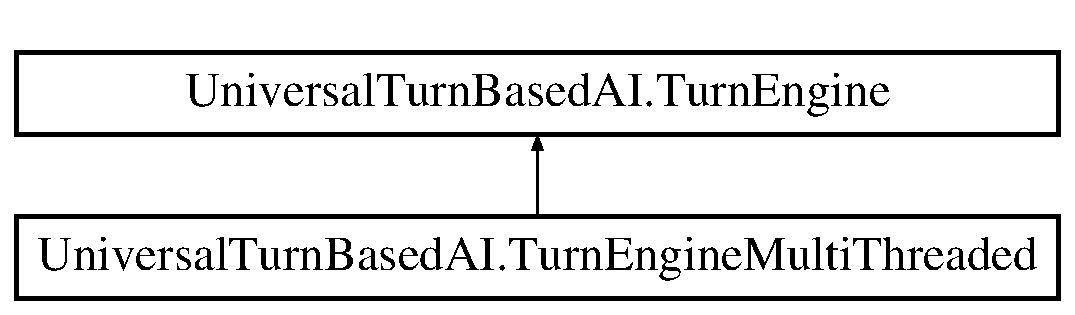
\includegraphics[height=2.000000cm]{class_universal_turn_based_a_i_1_1_turn_engine_multi_threaded}
\end{center}
\end{figure}
\subsection*{Public Member Functions}
\begin{DoxyCompactItemize}
\item 
\hyperlink{class_universal_turn_based_a_i_1_1_turn_engine_multi_threaded_a7159b2c6a0ffb898dc61ca2646399d4b}{Turn\+Engine\+Multi\+Threaded} (\hyperlink{interface_universal_turn_based_a_i_1_1_i_evaluator}{I\+Evaluator} eval, float time\+Limit, bool collect\+Stats=false)
\begin{DoxyCompactList}\small\item\em Initializes a new instance of the \hyperlink{class_universal_turn_based_a_i_1_1_turn_engine_multi_threaded}{Universal\+Turn\+Based\+A\+I.\+Turn\+Engine\+Multi\+Threaded} class with a time limit. Once the time limit has been reached the best turn found so far will be {\itshape best\+Turn}  \end{DoxyCompactList}\item 
\hyperlink{class_universal_turn_based_a_i_1_1_turn_engine_multi_threaded_a2c0825b1812b2c1b0065c1bf977423c4}{Turn\+Engine\+Multi\+Threaded} (\hyperlink{interface_universal_turn_based_a_i_1_1_i_evaluator}{I\+Evaluator} eval, int depth\+Limit, bool collect\+Stats=false)
\begin{DoxyCompactList}\small\item\em Initializes a new instance of the \hyperlink{class_universal_turn_based_a_i_1_1_turn_engine_multi_threaded}{Universal\+Turn\+Based\+A\+I.\+Turn\+Engine\+Multi\+Threaded} class with a depth limit. Searches the entire Game\+State tree up to the specific depth. The best turn found after the search will be {\itshape best\+Turn} . \end{DoxyCompactList}\item 
\hyperlink{class_universal_turn_based_a_i_1_1_turn_engine_multi_threaded_aba842ea4a30d4c58d1bb139aff873e8a}{Turn\+Engine\+Multi\+Threaded} (\hyperlink{interface_universal_turn_based_a_i_1_1_i_evaluator}{I\+Evaluator} eval, float time\+Limit, int depth\+Limit, bool collect\+Stats=false)
\begin{DoxyCompactList}\small\item\em Initializes a new instance of the \hyperlink{class_universal_turn_based_a_i_1_1_turn_engine_multi_threaded}{Universal\+Turn\+Based\+A\+I.\+Turn\+Engine\+Multi\+Threaded} class. \end{DoxyCompactList}\item 
\hypertarget{class_universal_turn_based_a_i_1_1_turn_engine_multi_threaded_a01bed3edbbe50d06f06e68b52af13c9c}{}override void {\bfseries Stop} ()\label{class_universal_turn_based_a_i_1_1_turn_engine_multi_threaded_a01bed3edbbe50d06f06e68b52af13c9c}

\end{DoxyCompactItemize}
\subsection*{Protected Member Functions}
\begin{DoxyCompactItemize}
\item 
override void \hyperlink{class_universal_turn_based_a_i_1_1_turn_engine_multi_threaded_a877d78f1b5b0f51ecf745bf5cf8fbb05}{Turn\+Search\+Delegate} (object state)
\begin{DoxyCompactList}\small\item\em A wrapper for the Minimax algorithm. Initialises the first branch of turns so that they can be given values and the best possible returned. Always generates at least one possible turns so that at least some sensible result can be returned. When the search is completed or timed out best\+Turn will be assigned to the best found turn. \end{DoxyCompactList}\end{DoxyCompactItemize}
\subsection*{Additional Inherited Members}


\subsection{Detailed Description}
A multi-\/threaded implementation of \hyperlink{class_universal_turn_based_a_i_1_1_turn_engine}{Turn\+Engine}. Uses the same search algorithm as \hyperlink{class_universal_turn_based_a_i_1_1_turn_engine_single_threaded}{Turn\+Engine\+Single\+Threaded} but runs each initial branch in a separate thread. 

This implementation may not be significantly faster than using \hyperlink{class_universal_turn_based_a_i_1_1_turn_engine_single_threaded}{Turn\+Engine\+Single\+Threaded} due to the overhead of managing multiple threads. May see an improvement if your Game\+State search tree is extremely wide i.\+e. in each state there is a very large number of possible moves to make.

\begin{DoxySeeAlso}{See also}
\hyperlink{class_universal_turn_based_a_i_1_1_turn_engine}{Turn\+Engine}, \hyperlink{class_universal_turn_based_a_i_1_1_turn_engine_single_threaded}{Turn\+Engine\+Single\+Threaded}


\end{DoxySeeAlso}


\subsection{Constructor \& Destructor Documentation}
\hypertarget{class_universal_turn_based_a_i_1_1_turn_engine_multi_threaded_a7159b2c6a0ffb898dc61ca2646399d4b}{}\index{Universal\+Turn\+Based\+A\+I\+::\+Turn\+Engine\+Multi\+Threaded@{Universal\+Turn\+Based\+A\+I\+::\+Turn\+Engine\+Multi\+Threaded}!Turn\+Engine\+Multi\+Threaded@{Turn\+Engine\+Multi\+Threaded}}
\index{Turn\+Engine\+Multi\+Threaded@{Turn\+Engine\+Multi\+Threaded}!Universal\+Turn\+Based\+A\+I\+::\+Turn\+Engine\+Multi\+Threaded@{Universal\+Turn\+Based\+A\+I\+::\+Turn\+Engine\+Multi\+Threaded}}
\subsubsection[{Turn\+Engine\+Multi\+Threaded}]{\setlength{\rightskip}{0pt plus 5cm}Universal\+Turn\+Based\+A\+I.\+Turn\+Engine\+Multi\+Threaded.\+Turn\+Engine\+Multi\+Threaded (
\begin{DoxyParamCaption}
\item[{{\bf I\+Evaluator}}]{eval, }
\item[{float}]{time\+Limit, }
\item[{bool}]{collect\+Stats = {\ttfamily false}}
\end{DoxyParamCaption}
)\hspace{0.3cm}{\ttfamily [inline]}}\label{class_universal_turn_based_a_i_1_1_turn_engine_multi_threaded_a7159b2c6a0ffb898dc61ca2646399d4b}


Initializes a new instance of the \hyperlink{class_universal_turn_based_a_i_1_1_turn_engine_multi_threaded}{Universal\+Turn\+Based\+A\+I.\+Turn\+Engine\+Multi\+Threaded} class with a time limit. Once the time limit has been reached the best turn found so far will be {\itshape best\+Turn}  


\begin{DoxyParams}{Parameters}
{\em eval} & The Evaluator\\
\hline
{\em time\+Limit} & The time limit, must be greater than 0\\
\hline
{\em collect\+Stats} & If set to {\ttfamily true} collect stats.\\
\hline
\end{DoxyParams}
\hypertarget{class_universal_turn_based_a_i_1_1_turn_engine_multi_threaded_a2c0825b1812b2c1b0065c1bf977423c4}{}\index{Universal\+Turn\+Based\+A\+I\+::\+Turn\+Engine\+Multi\+Threaded@{Universal\+Turn\+Based\+A\+I\+::\+Turn\+Engine\+Multi\+Threaded}!Turn\+Engine\+Multi\+Threaded@{Turn\+Engine\+Multi\+Threaded}}
\index{Turn\+Engine\+Multi\+Threaded@{Turn\+Engine\+Multi\+Threaded}!Universal\+Turn\+Based\+A\+I\+::\+Turn\+Engine\+Multi\+Threaded@{Universal\+Turn\+Based\+A\+I\+::\+Turn\+Engine\+Multi\+Threaded}}
\subsubsection[{Turn\+Engine\+Multi\+Threaded}]{\setlength{\rightskip}{0pt plus 5cm}Universal\+Turn\+Based\+A\+I.\+Turn\+Engine\+Multi\+Threaded.\+Turn\+Engine\+Multi\+Threaded (
\begin{DoxyParamCaption}
\item[{{\bf I\+Evaluator}}]{eval, }
\item[{int}]{depth\+Limit, }
\item[{bool}]{collect\+Stats = {\ttfamily false}}
\end{DoxyParamCaption}
)\hspace{0.3cm}{\ttfamily [inline]}}\label{class_universal_turn_based_a_i_1_1_turn_engine_multi_threaded_a2c0825b1812b2c1b0065c1bf977423c4}


Initializes a new instance of the \hyperlink{class_universal_turn_based_a_i_1_1_turn_engine_multi_threaded}{Universal\+Turn\+Based\+A\+I.\+Turn\+Engine\+Multi\+Threaded} class with a depth limit. Searches the entire Game\+State tree up to the specific depth. The best turn found after the search will be {\itshape best\+Turn} . 


\begin{DoxyParams}{Parameters}
{\em eval} & Eval.\\
\hline
{\em depth\+Limit} & Depth limit, must be at least 1\\
\hline
{\em collect\+Stats} & If set to {\ttfamily true} collect stats.\\
\hline
\end{DoxyParams}
\hypertarget{class_universal_turn_based_a_i_1_1_turn_engine_multi_threaded_aba842ea4a30d4c58d1bb139aff873e8a}{}\index{Universal\+Turn\+Based\+A\+I\+::\+Turn\+Engine\+Multi\+Threaded@{Universal\+Turn\+Based\+A\+I\+::\+Turn\+Engine\+Multi\+Threaded}!Turn\+Engine\+Multi\+Threaded@{Turn\+Engine\+Multi\+Threaded}}
\index{Turn\+Engine\+Multi\+Threaded@{Turn\+Engine\+Multi\+Threaded}!Universal\+Turn\+Based\+A\+I\+::\+Turn\+Engine\+Multi\+Threaded@{Universal\+Turn\+Based\+A\+I\+::\+Turn\+Engine\+Multi\+Threaded}}
\subsubsection[{Turn\+Engine\+Multi\+Threaded}]{\setlength{\rightskip}{0pt plus 5cm}Universal\+Turn\+Based\+A\+I.\+Turn\+Engine\+Multi\+Threaded.\+Turn\+Engine\+Multi\+Threaded (
\begin{DoxyParamCaption}
\item[{{\bf I\+Evaluator}}]{eval, }
\item[{float}]{time\+Limit, }
\item[{int}]{depth\+Limit, }
\item[{bool}]{collect\+Stats = {\ttfamily false}}
\end{DoxyParamCaption}
)\hspace{0.3cm}{\ttfamily [inline]}}\label{class_universal_turn_based_a_i_1_1_turn_engine_multi_threaded_aba842ea4a30d4c58d1bb139aff873e8a}


Initializes a new instance of the \hyperlink{class_universal_turn_based_a_i_1_1_turn_engine_multi_threaded}{Universal\+Turn\+Based\+A\+I.\+Turn\+Engine\+Multi\+Threaded} class. 


\begin{DoxyParams}{Parameters}
{\em eval} & The \hyperlink{interface_universal_turn_based_a_i_1_1_i_evaluator}{I\+Evaluator} to use\\
\hline
{\em time\+Limit} & Time limit in seconds. Must be greater than 0\\
\hline
{\em depth\+Limit} & Depth limit or maximum \char`\"{}ply\char`\"{}. Must be at least 1\\
\hline
{\em collect\+Stats} & If set to {\ttfamily true} collect stats.\\
\hline
\end{DoxyParams}


\subsection{Member Function Documentation}
\hypertarget{class_universal_turn_based_a_i_1_1_turn_engine_multi_threaded_a877d78f1b5b0f51ecf745bf5cf8fbb05}{}\index{Universal\+Turn\+Based\+A\+I\+::\+Turn\+Engine\+Multi\+Threaded@{Universal\+Turn\+Based\+A\+I\+::\+Turn\+Engine\+Multi\+Threaded}!Turn\+Search\+Delegate@{Turn\+Search\+Delegate}}
\index{Turn\+Search\+Delegate@{Turn\+Search\+Delegate}!Universal\+Turn\+Based\+A\+I\+::\+Turn\+Engine\+Multi\+Threaded@{Universal\+Turn\+Based\+A\+I\+::\+Turn\+Engine\+Multi\+Threaded}}
\subsubsection[{Turn\+Search\+Delegate}]{\setlength{\rightskip}{0pt plus 5cm}override void Universal\+Turn\+Based\+A\+I.\+Turn\+Engine\+Multi\+Threaded.\+Turn\+Search\+Delegate (
\begin{DoxyParamCaption}
\item[{object}]{state}
\end{DoxyParamCaption}
)\hspace{0.3cm}{\ttfamily [inline]}, {\ttfamily [protected]}, {\ttfamily [virtual]}}\label{class_universal_turn_based_a_i_1_1_turn_engine_multi_threaded_a877d78f1b5b0f51ecf745bf5cf8fbb05}


A wrapper for the Minimax algorithm. Initialises the first branch of turns so that they can be given values and the best possible returned. Always generates at least one possible turns so that at least some sensible result can be returned. When the search is completed or timed out best\+Turn will be assigned to the best found turn. 

For each initial turn this created a new \hyperlink{class_universal_turn_based_a_i_1_1_minimax_worker}{Minimax\+Worker} is created and added to a Thread\+Pool. Then it waits for each thread to finish or a time out. \begin{DoxySeeAlso}{See also}
\hyperlink{class_universal_turn_based_a_i_1_1_minimax_worker}{Minimax\+Worker}


\end{DoxySeeAlso}



\begin{DoxyParams}{Parameters}
{\em state} & The starting state\\
\hline
\end{DoxyParams}


Implements \hyperlink{class_universal_turn_based_a_i_1_1_turn_engine}{Universal\+Turn\+Based\+A\+I.\+Turn\+Engine}.



The documentation for this class was generated from the following file\+:\begin{DoxyCompactItemize}
\item 
Generic\+Turn\+Based\+A\+I/Turn\+Engine\+Multi\+Threaded.\+cs\end{DoxyCompactItemize}

\hypertarget{class_universal_turn_based_a_i_1_1_turn_engine_single_threaded}{}\section{Universal\+Turn\+Based\+A\+I.\+Turn\+Engine\+Single\+Threaded Class Reference}
\label{class_universal_turn_based_a_i_1_1_turn_engine_single_threaded}\index{Universal\+Turn\+Based\+A\+I.\+Turn\+Engine\+Single\+Threaded@{Universal\+Turn\+Based\+A\+I.\+Turn\+Engine\+Single\+Threaded}}


A single threaded implementation of \hyperlink{class_universal_turn_based_a_i_1_1_turn_engine}{Turn\+Engine}. Uses an implementation of the Minimax algorithm with Alpha-\/\+Beta pruning.  


Inheritance diagram for Universal\+Turn\+Based\+A\+I.\+Turn\+Engine\+Single\+Threaded\+:\begin{figure}[H]
\begin{center}
\leavevmode
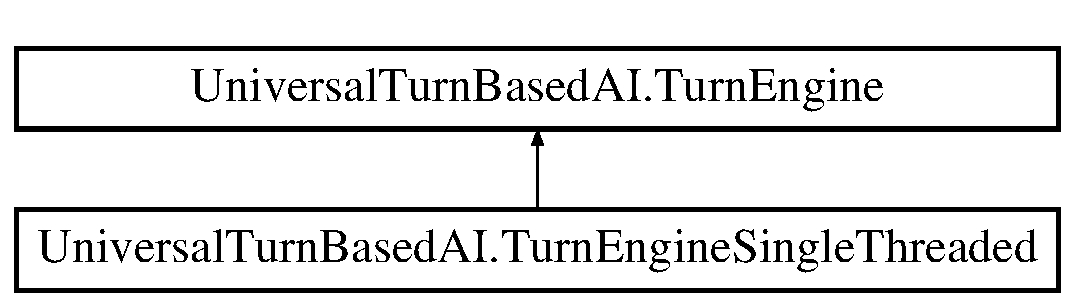
\includegraphics[height=2.000000cm]{class_universal_turn_based_a_i_1_1_turn_engine_single_threaded}
\end{center}
\end{figure}
\subsection*{Public Member Functions}
\begin{DoxyCompactItemize}
\item 
\hyperlink{class_universal_turn_based_a_i_1_1_turn_engine_single_threaded_a4b4e3d37f9646bf0f5bceb64d1ea560b}{Turn\+Engine\+Single\+Threaded} (\hyperlink{interface_universal_turn_based_a_i_1_1_i_evaluator}{I\+Evaluator} eval, float time\+Limit, bool collect\+Stats=false)
\begin{DoxyCompactList}\small\item\em Initializes a new instance of the \hyperlink{class_universal_turn_based_a_i_1_1_turn_engine_single_threaded}{Universal\+Turn\+Based\+A\+I.\+Turn\+Engine\+Single\+Threaded} class with a time limit. Once the time limit has been reached the best turn found so far will be {\itshape best\+Turn}  \end{DoxyCompactList}\item 
\hyperlink{class_universal_turn_based_a_i_1_1_turn_engine_single_threaded_a85a136e7e4a46bb4ff5283b2a1b7da8e}{Turn\+Engine\+Single\+Threaded} (\hyperlink{interface_universal_turn_based_a_i_1_1_i_evaluator}{I\+Evaluator} eval, int depth\+Limit, bool collect\+Stats=false)
\begin{DoxyCompactList}\small\item\em Initializes a new instance of the \hyperlink{class_universal_turn_based_a_i_1_1_turn_engine_single_threaded}{Universal\+Turn\+Based\+A\+I.\+Turn\+Engine\+Single\+Threaded} class with a depth limit. Searches the entire Game\+State tree up to the specific depth. The best turn found after the search will be {\itshape best\+Turn} . \end{DoxyCompactList}\item 
\hyperlink{class_universal_turn_based_a_i_1_1_turn_engine_single_threaded_abb6589d9134a6a427d07d43319e54823}{Turn\+Engine\+Single\+Threaded} (\hyperlink{interface_universal_turn_based_a_i_1_1_i_evaluator}{I\+Evaluator} eval, float time\+Limit, int depth\+Limit, bool collect\+Stats=false)
\begin{DoxyCompactList}\small\item\em Initializes a new instance of the \hyperlink{class_universal_turn_based_a_i_1_1_turn_engine_single_threaded}{Universal\+Turn\+Based\+A\+I.\+Turn\+Engine\+Single\+Threaded} class with both a time and depth limit. \end{DoxyCompactList}\end{DoxyCompactItemize}
\subsection*{Protected Member Functions}
\begin{DoxyCompactItemize}
\item 
override void \hyperlink{class_universal_turn_based_a_i_1_1_turn_engine_single_threaded_a2ae467b6b27ec5e2dfe1d033c86ea4d8}{Turn\+Search\+Delegate} (object state)
\begin{DoxyCompactList}\small\item\em A wrapper for the Minimax algorithm. Initialises the first branch of turns so that they can be given values and the best possible returned. Always generates at least one possible turns so that at least some sensible result can be returned. When the search is completed or timed out best\+Turn will be assigned to the best found turn. \end{DoxyCompactList}\end{DoxyCompactItemize}
\subsection*{Additional Inherited Members}


\subsection{Detailed Description}
A single threaded implementation of \hyperlink{class_universal_turn_based_a_i_1_1_turn_engine}{Turn\+Engine}. Uses an implementation of the Minimax algorithm with Alpha-\/\+Beta pruning. 

\begin{DoxySeeAlso}{See also}
\hyperlink{class_universal_turn_based_a_i_1_1_turn_engine}{Turn\+Engine}, \hyperlink{class_universal_turn_based_a_i_1_1_turn_engine_multi_threaded}{Turn\+Engine\+Multi\+Threaded}


\end{DoxySeeAlso}


\subsection{Constructor \& Destructor Documentation}
\hypertarget{class_universal_turn_based_a_i_1_1_turn_engine_single_threaded_a4b4e3d37f9646bf0f5bceb64d1ea560b}{}\index{Universal\+Turn\+Based\+A\+I\+::\+Turn\+Engine\+Single\+Threaded@{Universal\+Turn\+Based\+A\+I\+::\+Turn\+Engine\+Single\+Threaded}!Turn\+Engine\+Single\+Threaded@{Turn\+Engine\+Single\+Threaded}}
\index{Turn\+Engine\+Single\+Threaded@{Turn\+Engine\+Single\+Threaded}!Universal\+Turn\+Based\+A\+I\+::\+Turn\+Engine\+Single\+Threaded@{Universal\+Turn\+Based\+A\+I\+::\+Turn\+Engine\+Single\+Threaded}}
\subsubsection[{Turn\+Engine\+Single\+Threaded}]{\setlength{\rightskip}{0pt plus 5cm}Universal\+Turn\+Based\+A\+I.\+Turn\+Engine\+Single\+Threaded.\+Turn\+Engine\+Single\+Threaded (
\begin{DoxyParamCaption}
\item[{{\bf I\+Evaluator}}]{eval, }
\item[{float}]{time\+Limit, }
\item[{bool}]{collect\+Stats = {\ttfamily false}}
\end{DoxyParamCaption}
)\hspace{0.3cm}{\ttfamily [inline]}}\label{class_universal_turn_based_a_i_1_1_turn_engine_single_threaded_a4b4e3d37f9646bf0f5bceb64d1ea560b}


Initializes a new instance of the \hyperlink{class_universal_turn_based_a_i_1_1_turn_engine_single_threaded}{Universal\+Turn\+Based\+A\+I.\+Turn\+Engine\+Single\+Threaded} class with a time limit. Once the time limit has been reached the best turn found so far will be {\itshape best\+Turn}  


\begin{DoxyParams}{Parameters}
{\em eval} & The Evaluator\\
\hline
{\em time\+Limit} & The time limit, must be greater than 0\\
\hline
{\em collect\+Stats} & If set to {\ttfamily true} collect stats.\\
\hline
\end{DoxyParams}
\hypertarget{class_universal_turn_based_a_i_1_1_turn_engine_single_threaded_a85a136e7e4a46bb4ff5283b2a1b7da8e}{}\index{Universal\+Turn\+Based\+A\+I\+::\+Turn\+Engine\+Single\+Threaded@{Universal\+Turn\+Based\+A\+I\+::\+Turn\+Engine\+Single\+Threaded}!Turn\+Engine\+Single\+Threaded@{Turn\+Engine\+Single\+Threaded}}
\index{Turn\+Engine\+Single\+Threaded@{Turn\+Engine\+Single\+Threaded}!Universal\+Turn\+Based\+A\+I\+::\+Turn\+Engine\+Single\+Threaded@{Universal\+Turn\+Based\+A\+I\+::\+Turn\+Engine\+Single\+Threaded}}
\subsubsection[{Turn\+Engine\+Single\+Threaded}]{\setlength{\rightskip}{0pt plus 5cm}Universal\+Turn\+Based\+A\+I.\+Turn\+Engine\+Single\+Threaded.\+Turn\+Engine\+Single\+Threaded (
\begin{DoxyParamCaption}
\item[{{\bf I\+Evaluator}}]{eval, }
\item[{int}]{depth\+Limit, }
\item[{bool}]{collect\+Stats = {\ttfamily false}}
\end{DoxyParamCaption}
)\hspace{0.3cm}{\ttfamily [inline]}}\label{class_universal_turn_based_a_i_1_1_turn_engine_single_threaded_a85a136e7e4a46bb4ff5283b2a1b7da8e}


Initializes a new instance of the \hyperlink{class_universal_turn_based_a_i_1_1_turn_engine_single_threaded}{Universal\+Turn\+Based\+A\+I.\+Turn\+Engine\+Single\+Threaded} class with a depth limit. Searches the entire Game\+State tree up to the specific depth. The best turn found after the search will be {\itshape best\+Turn} . 


\begin{DoxyParams}{Parameters}
{\em eval} & Eval.\\
\hline
{\em depth\+Limit} & Depth limit, must be at least 1\\
\hline
{\em collect\+Stats} & If set to {\ttfamily true} collect stats.\\
\hline
\end{DoxyParams}
\hypertarget{class_universal_turn_based_a_i_1_1_turn_engine_single_threaded_abb6589d9134a6a427d07d43319e54823}{}\index{Universal\+Turn\+Based\+A\+I\+::\+Turn\+Engine\+Single\+Threaded@{Universal\+Turn\+Based\+A\+I\+::\+Turn\+Engine\+Single\+Threaded}!Turn\+Engine\+Single\+Threaded@{Turn\+Engine\+Single\+Threaded}}
\index{Turn\+Engine\+Single\+Threaded@{Turn\+Engine\+Single\+Threaded}!Universal\+Turn\+Based\+A\+I\+::\+Turn\+Engine\+Single\+Threaded@{Universal\+Turn\+Based\+A\+I\+::\+Turn\+Engine\+Single\+Threaded}}
\subsubsection[{Turn\+Engine\+Single\+Threaded}]{\setlength{\rightskip}{0pt plus 5cm}Universal\+Turn\+Based\+A\+I.\+Turn\+Engine\+Single\+Threaded.\+Turn\+Engine\+Single\+Threaded (
\begin{DoxyParamCaption}
\item[{{\bf I\+Evaluator}}]{eval, }
\item[{float}]{time\+Limit, }
\item[{int}]{depth\+Limit, }
\item[{bool}]{collect\+Stats = {\ttfamily false}}
\end{DoxyParamCaption}
)\hspace{0.3cm}{\ttfamily [inline]}}\label{class_universal_turn_based_a_i_1_1_turn_engine_single_threaded_abb6589d9134a6a427d07d43319e54823}


Initializes a new instance of the \hyperlink{class_universal_turn_based_a_i_1_1_turn_engine_single_threaded}{Universal\+Turn\+Based\+A\+I.\+Turn\+Engine\+Single\+Threaded} class with both a time and depth limit. 


\begin{DoxyParams}{Parameters}
{\em eval} & The \hyperlink{interface_universal_turn_based_a_i_1_1_i_evaluator}{I\+Evaluator} to use\\
\hline
{\em time\+Limit} & Time limit in seconds. Must be greater than 0\\
\hline
{\em depth\+Limit} & Depth limit or maximum \char`\"{}ply\char`\"{}. Must be at least 1\\
\hline
{\em collect\+Stats} & If set to {\ttfamily true} collect stats.\\
\hline
\end{DoxyParams}


\subsection{Member Function Documentation}
\hypertarget{class_universal_turn_based_a_i_1_1_turn_engine_single_threaded_a2ae467b6b27ec5e2dfe1d033c86ea4d8}{}\index{Universal\+Turn\+Based\+A\+I\+::\+Turn\+Engine\+Single\+Threaded@{Universal\+Turn\+Based\+A\+I\+::\+Turn\+Engine\+Single\+Threaded}!Turn\+Search\+Delegate@{Turn\+Search\+Delegate}}
\index{Turn\+Search\+Delegate@{Turn\+Search\+Delegate}!Universal\+Turn\+Based\+A\+I\+::\+Turn\+Engine\+Single\+Threaded@{Universal\+Turn\+Based\+A\+I\+::\+Turn\+Engine\+Single\+Threaded}}
\subsubsection[{Turn\+Search\+Delegate}]{\setlength{\rightskip}{0pt plus 5cm}override void Universal\+Turn\+Based\+A\+I.\+Turn\+Engine\+Single\+Threaded.\+Turn\+Search\+Delegate (
\begin{DoxyParamCaption}
\item[{object}]{state}
\end{DoxyParamCaption}
)\hspace{0.3cm}{\ttfamily [inline]}, {\ttfamily [protected]}, {\ttfamily [virtual]}}\label{class_universal_turn_based_a_i_1_1_turn_engine_single_threaded_a2ae467b6b27ec5e2dfe1d033c86ea4d8}


A wrapper for the Minimax algorithm. Initialises the first branch of turns so that they can be given values and the best possible returned. Always generates at least one possible turns so that at least some sensible result can be returned. When the search is completed or timed out best\+Turn will be assigned to the best found turn. 


\begin{DoxyParams}{Parameters}
{\em state} & The starting state\\
\hline
\end{DoxyParams}


Implements \hyperlink{class_universal_turn_based_a_i_1_1_turn_engine}{Universal\+Turn\+Based\+A\+I.\+Turn\+Engine}.



The documentation for this class was generated from the following file\+:\begin{DoxyCompactItemize}
\item 
Generic\+Turn\+Based\+A\+I/Turn\+Engine\+Single\+Threaded.\+cs\end{DoxyCompactItemize}

%--- End generated contents ---

% Index
\backmatter
\newpage
\phantomsection
\clearemptydoublepage
\addcontentsline{toc}{chapter}{Index}
\printindex

\end{document}
